\documentclass[a4paper, twoside, 12pt]{book}

\usepackage{fontspec}
\usepackage[spanish, english, french]{babel}

\usepackage[utf8]{inputenc}
\usepackage[T1]{fontenc}

%Configuration de la mise en page
%Menus des annexes
\usepackage{appendix}

%Gestion des images
\usepackage{graphicx}
\usepackage{wrapfig}
\addto\captionsfrench{\def\figurename{Image}}
\addto\captionsfrench{\def\tablename{Tableau}}

%Modifier taille légende des images
\usepackage[font=small]{caption}

%Note de bas de page
\counterwithout*{footnote}{chapter}

% Éléments de mise en page (marge de 2,5 cm, alinéa en début de paragraphe 1cm, interligne 1,5)
\usepackage{setspace}
\onehalfspacing
\setlength{\parindent}{1cm}
\usepackage[a4paper,margin=2.5cm]{geometry}
%Colonnes
\usepackage{paracol}

%%barrer du texte
\usepackage{soul}

%TABLEAU
\usepackage{longtable}
%pour mode paysage
\usepackage{lscape}
%Pour paysage dans le pdf
\usepackage{pdflscape}
%Utiliser couleurs dans un tableau
\usepackage{colortbl}
%gestion avancée des couleurs. On met nom de la couleur puis !pourcentage
\usepackage{xcolor}
%Séparer une cellule en 2
\usepackage{diagbox}

\usepackage{epigraph}

%Pour avoir liens dans document (externes ou internes)
\usepackage{hyperref}
\hypersetup{pdfauthor={Lise Bernard},pdftitle={memoire_M1}, pdfborder=0 0 0}


%% Commande écriture inclusive
\newcommand{\inclusive}[1]{$\cdot${#1}}
\newcommand{\inclusives}[1]{$\cdot${#1}$\cdot${s}}

%commande siècle
\newcommand{\siecle}[1]{\textsc{#1}\textsuperscript{e} siècle}

%Commande pour vider le titre courant et pagination des pages vides (l'insérer sur page que l'on veut vider)
\newcommand{\clearemptydoublepage}{
	\newpage{\pagestyle{empty}\cleardoublepage}}

% Listes
\usepackage{enumerate}
\usepackage{enumitem}


%%Bibliographie
% Pour avoir guillemets français dans biblio
\usepackage[autostyle]{csquotes} 
%paquet gestion biblio
\usepackage[backend=biber, sorting=nyt,maxbibnames=10,style=enc]{biblatex}

%Préambule
\addbibresource{biblio/TextAnd.bib}
\addbibresource{biblio/TextNum.bib}
\addbibresource{biblio/projets.bib}

\DeclareSourcemap{
	\maps[datatype=bibtex]{
		\map[overwrite]{
			\perdatasource{biblio/TextAnd.bib}
			\step[fieldset=keywords, fieldvalue={,TextAnd}, append]
		}
        \map[overwrite]{
			\perdatasource{biblio/TextNum.bib}
			\step[fieldset=keywords, fieldvalue={,textnum}, append]
		}
        \map[overwrite]{
			\perdatasource{biblio/projets.bib}
			\step[fieldset=keywords, fieldvalue={,Pjet}, append]
		}
	}
}


\begin{document}
\frontmatter

\begin{titlepage}
\begin{center}

\bigskip

\begin{large}
UNIVERSITÉ PARIS, SCIENCES \& LETTRES
\end{large}

\begin{center}\rule{2cm}{0.02cm}\end{center}

\bigskip
\bigskip
\bigskip
\begin{Large}
\textbf{Lise Bernard}\\
\end{Large}
\begin{normalsize}
\textit{Diplômée de Master en anthropologie de l'Amérique latine}\\
\end{normalsize}

\bigskip
\bigskip
\bigskip
\bigskip
\bigskip

\begin{LARGE}
\textbf{La compréhension des motifs tissés dans les Andes : une approche par la détection automatique}\\
\end{LARGE}

\bigskip
\bigskip
\bigskip
\vfill

\begin{large}
Mémoire de première année du master\\
\og Humanités Numériques \fg{} \\
\bigskip
Juin 2023
\end{large}

\end{center}
\end{titlepage}


\section*{Remerciements}

\vspace{30pt}

    Tout d'abord, je voudrais remercier mes deux directeurs de recherche. Mme Astrid Castres qui a pris le temps de se plonger dans les Humanités Numériques, et M. Daniel Stockholm pour son aide dans la découverte de l'analyse de l'image.

\begin{center}
    ***
\end{center}

    Je tiens aussi à remercier les professeurs de l'École Nationale des Chartes auprès desquels je me forme aux Humanités Numériques dans un cadre bienveillant et stimulant.

\begin{center}
    ***
\end{center}

    Je suis très reconnaissante envers mes camarades de classe, sans qui cette année n'aurait pas été la même.
    
\begin{center}
    ***
\end{center}

    Bien évidemment merci aux ami\inclusives{e}, toutes celles et tous ceux qui ont rendu ces mois de travail ardu, plus légers. Une pensée particulière pour Alice, la meilleure relectrice malgré ses utilisations douteuses des expressions françaises. \textit{!`Te deseo lo mejor!}



% table des matières
\renewcommand{\contentsname}{Sommaire}
\tableofcontents
\markboth{}{}

\clearpage

\mainmatter

\chapter*{Introduction}
\addcontentsline{toc}{chapter}{Introduction}

Au Pérou, une multitude de textiles a été retrouvée lors des nombreuses fouilles archéologiques qui ont eu lieu depuis le milieu du 20e siècle\footnote{\cite{onealeTextilePeriodsAncient1930}}. Si ces découvertes sont possible c'est notamment grâce au climat désertique le long de la côte péruvienne qui offre des conditions de conservation idéale pour les fibres animales et végétales qui composent les pièces textiles\footnote{\cite{desrosiersTechniquesTissageOntelles2010}}. À l'inverse, les civilisations de la Cordillère des Andes (ou \textit{Sierra}) ont été productrices de textiles, mais le climat humide et froid en altitude n'a pas permis leur conservation --- à part quelques échantillons retrouvés sur des momies découvertes au-dessus de 5000 mètres d'altitude et dont les vêtements ont été conservés par la congélation\footnote{\cite{abalderussoArteTextilIncaico2010}}--- .
\noindent Ces textiles sont des pièces qui apparaissent sur la longue durée, puisqu'il s'agit d'un témoignage de cultures matérielles s'étendant sur plus d'un millénaire.

\begin{figure}[!h]
    \centering
    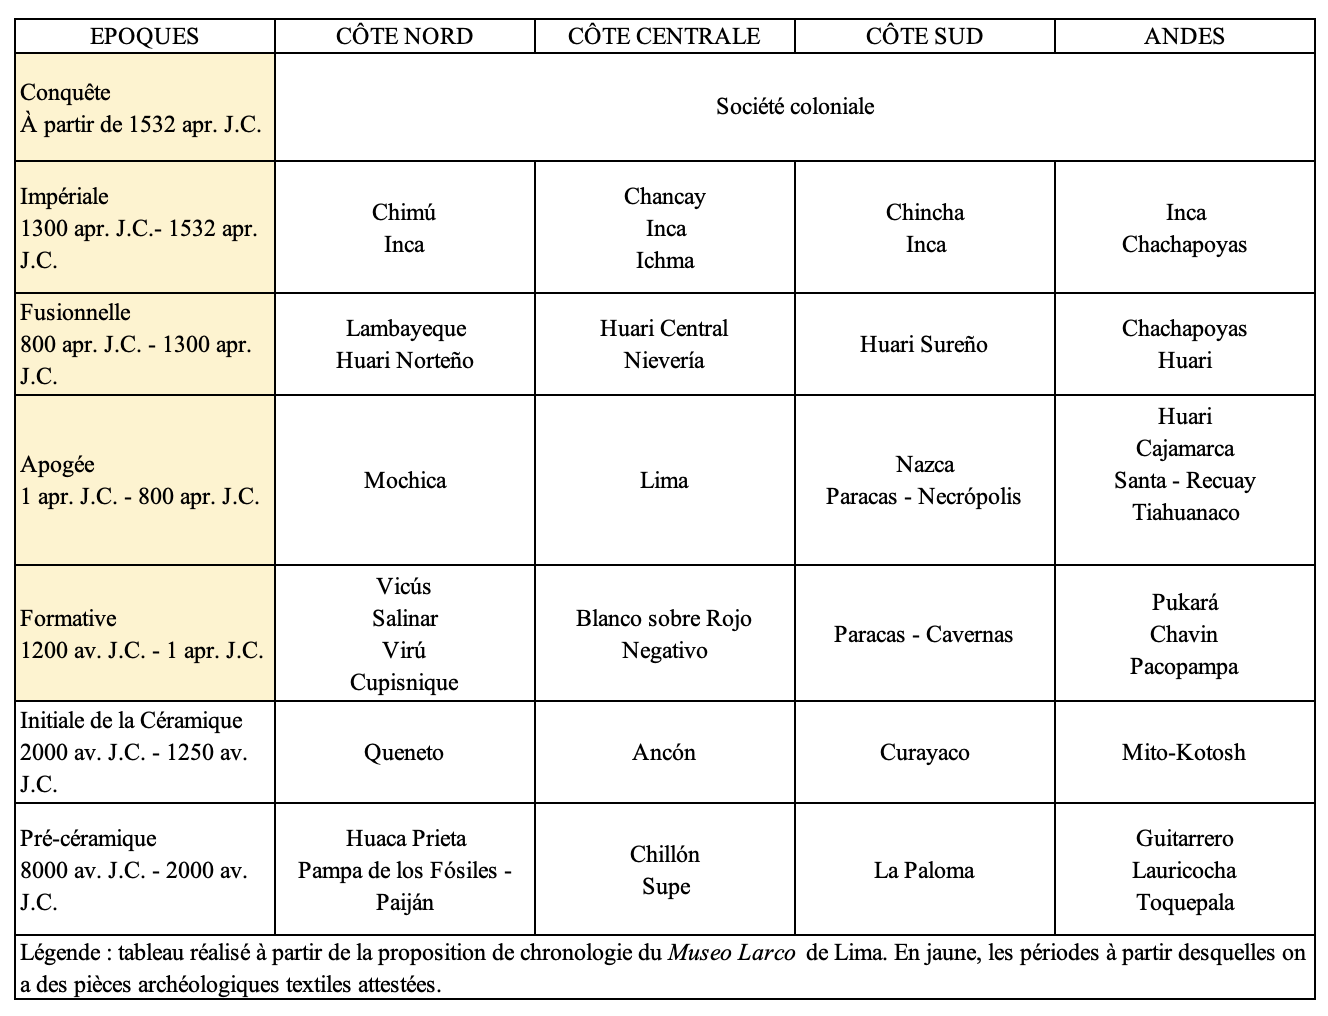
\includegraphics[width=12cm]{images/civiPerou.png}
    \caption{Tableau des civilisations péruviennes jusqu'à la colonisation espagnole.}
    \label{fig:1}
\end{figure}

Comme le souligne Jorge Sebastián Lozano et son équipe, \og Le patrimoine textile est un des nombreux parents pauvres dans la grande famille du patrimoine culturel \fg \footcite[p.~76]{sebastianlozanoCatalogosMuseoGran2020} et il a encore beaucoup à nous apprendre. Ma recherche porte sur les textiles archéologiques et ethnographiques péruviens en tant qu'objets dynamiques et indicateurs des évolutions des motifs et des techniques. 


\section*{État de l'art}
\addcontentsline{toc}{section}{État de l'art}

\subsection*{La foisonnante étude des textiles andins}
\addcontentsline{toc}{subsection}{La foisonnante étude des textiles andins}

Dans les années 1930, les études américanistes se concentrent sur les découvertes archéologiques préhispaniques, y compris sur le textile. 
Lila O'Neale et Alfred Kroeber proposent ainsi des premières pistes d'analyse des textiles archéologiques découverts sur la côte péruvienne au début du \siecle{xx}\footcite{onealeTextilePeriodsAncient1930}. Leur ouvrage se compose principalement de planches photographiques.
En France, Raoul D'Harcourt, précurseur de l'ethnographie andiniste française, propose la première analyse des textiles archéologiques du Pérou et de leurs techniques en 1934\footcite{harcourtTextilesAnciensPerou2008}. Il s'applique à montrer la complexité des techniques utilisées par les populations préhispaniques et en propose une typologie. 
Ainsi, l'anthropologie s'est longtemps intéressée au textile en tant qu'objet et, surtout, comme un objet appartenant au passé, produit par des populations disparues. À cette période, certaines techniques textiles de ces populations étaient toujours existantes dans les communautés indigènes, notamment dans les Andes. Toutefois, l'intérêt pour les textiles ethnographiques apparaît plus tard dans la discipline anthropologique --- nous y reviendrons ---.

Une grande partie de l'analyse du textile, y compris dans le champ andiniste, consiste alors à penser la classification des artefacts. André Leroi-Gourhan, en 1943, dans sa classification générale des techniques, analyse les moyens de productions textiles, y compris ceux utilisés dans les Andes.
Sophie Desrosiers, spécialiste française des textiles andins, se montre critique face à cette classification. Elle souligne que Leroi-Gourhan se contredit dans son étude du textile puisqu'il promeut une classification des techniques à partir des matières premières, mais, pour le textile, il classifie les pièces selon l'assemblage des fibres et non leur composition. Par ailleurs, elle souligne qu'il ne faut pas oublier que les textiles sont des constructions en trois dimensions, et non pas juste un plan composé de motifs, large tendance dans l'approche des textiles. L'ouvrage de référence en matière de classification textile est encore aujourd'hui \textit{The Primary Structure of Fabrics} au sein duquel Irene Emery propose une classification des techniques selon l'entrecroisement des fils, accompagnée de photographies\footcite{emeryPrimaryStructuresFabrics1995}. Elle prend d'ailleurs des exemples d'armures textiles à partir de pièces archéologiques découvertes au Pérou. Nous pouvons aussi nous référer à l'ouvrage d'Annemarie Seiler-Badinger pour une classification généraliste du textile selon son mode de production\footcite{seiler-baldingerTextilesClassificationTechniques1995}\footnote{Pour le débat sur les différentes proposition de classification textile, voir : \cite{balfetOuSontClassifications1988}}.

Dans les années 1980, on assiste à une reviviscence de l'analyse des textiles. À partir de cette décennie, les chercheurs et chercheuses s'intéressent moins aux textiles archéologiques et à leurs structures qu'aux textiles récents comme outils de compréhension des textiles archéologiques. Ce courant développe une classification selon les techniques contemporaines observables, applicable à la fois aux textiles ethnographiques et aux textiles archéologiques, et un fort intérêt est porté aux données des sources historiques. Par exemple, Sophie Desrosiers propose la reconstitution d'une ceinture dont la construction est présentée dans une chronique de Fray Martín de Murúa  au \siecle{xvii}, \textit{Historia del origen y genealogía de los Reyes Incas del Perú}\footcite{desrosiersExperienceTechnologieReconstruction1986}. Ainsi, le champ se complexifie : les analyses approfondissent les techniques mais aussi le lien entre textiles, cosmologie andine et pratiques sociales locales. De nouveaux thèmes émergent comme la comparaison interculturelle, les classifications linguistiques des textiles ou l'approche par l'anthropologie sociale et culturelle. Les chercheuses et les chercheurs produisent des monographies ethnographiques qui se concentrent sur les textiles contemporains. Les études interdisciplinaires du textile andin se développent. 
Ainsi, Denise Arnold et Elvira Espejo complètent la connaissance des pièces andines par une approche linguistique des textiles et de leur fabrication\footcite{arnoldHaciaTerminologiaAndina2011}. En effet, les textiles andins sont, bien souvent, fabriqués par des personnes quechuaphones ou aymaraphones\footnote{Le quechua et l'aymara sont les deux langues amérindiennes les plus parlées dans les Andes. À elles deux, elles comptent plus de 10 millions de locuteurs répartis entre le Pérou, la Bolivie, l'Équateur, le Chili et l'Argentine.}. L'analyse de la langue permettrait alors de comprendre les logiques de tissage des femmes, et inversement. Cette approche par la langue avait d'abord été développée par Verónica Cereceda à propos des \textit{talegas} (type de sacs) d'Isluga (Bolivie)\footcite{cerecedaSemiologieTissusAndins1978}. Plus récemment, Denise Arnold et Elvira Espejo ont elles aussi proposé une classification des techniques textiles mais cette fois-ci spécialement dédiée aux textiles andins, essayant de saisir la multitude de techniques qui étaient ou sont encore présentes sur le territoire péruvien. Elles ancrent leur ouvrage comme un outil pour les tisserand\inclusives{e} contemporain\inclusives{e} pour \og offrir ici des informations auparavant disponibles pour les spécialistes et les rendre plus accessibles, dans l'espoir de contribuer au sauvetage et à la revalorisation d'une partie de la complexité technique et technologique antérieure\footnote{\cite[p.~8]{arnoldCienciaTejerAndes2019} \textquotedblleft \textit{ofrecer aquí una información previamente disponible a los especialistas y hacerla más accesible, con la esperanza de contribuir a que se rescate y se revalorice una parte de la complejidad técnica y tecnológica anterior}''}.\fg \\

L'histoire est également un domaine fertile pour comprendre l'inscription du textile dans la société péruvienne. C'est une pratique très ancienne au Pérou, les preuves archéologiques ne manquent pas et dès les premières chroniques\footnote{Le terme de chronique renvoie aux ouvrages rédigés par des colons ou par des métis à partir de la période coloniale. Les chroniques contiennent des descriptions de la colonisation, du mode de vie des habitants colonisés, de la géographies ou de la faune et de la flore locale, ainsi que des récits historiques rapportés par les populations locales.} la présence du textile est soulignée.

Comme nous l'avons vu, l'anthropologie --- mais aussi l'archéologie --- a fourni de nombreuses analyses des textiles andins préhispaniques. Pour autant, il reste des mystères comme, par exemple, la signification de certains \textit{khipus} sur laquelle de nombreux archéologues ou anthropologues travaillent encore\footnote{Les \textit{khipus} sont des ensembles de cordelettes, nouées entre elles et sur elles-mêmes, qui permettaient de tenir une comptabilité ou bien d'envoyer des messages. Ils sont extensivement utilisés au cours de l'Empire Inca.}. Les découvertes de pièces archéologiques continuent, notamment certaines momies dont les tombes sont dévoilées par la fonte des glaciers\footcite{abalderussoArteTextilIncaico2010}. 

Cependant, les pratiques textiles dépendent aussi de l'histoire de la circulation transatlantique à partir de la colonisation du continent. Les travaux d'Elena Phipps montrent en effet l'importance du commerce textile entre la métropole et ses colonies\footcite{phippsIberianGlobe2013}. Une grande partie des textiles acquis par le tribut est ainsi exportée et des artisan\inclusives{e} locaux sont désigné\inclusives{e} pour produire les textiles destinés à la royauté espagnole. Mais la circulation des textiles se fait aussi depuis la métropole vers les colonies : \og les textiles, parmi tous les objets, sont ceux qui ont été les plus envoyés depuis l'Espagne vers les Amériques \fg \footnote{\cite[p.~33]{phippsIberianGlobe2013} \textit{\textquotedblleft More textiles were shipped from Spain to Americas than any other items''}}. Les colonies sont donc une zone de débouchés pour une partie de la production textile espagnole (notamment la soie espagnole et les fils métalliques). La circulation de l'Espagne vers les colonies se fait aussi par l'arrivée d'artisans européens, notamment de brodeurs qui s'organisent en guildes et qui transmettent leurs savoirs. Ainsi, l'iconographie textile du Pérou s'hybride rapidement à la fois entre communautés mais aussi par l'influence des colonisateurs\footcite{solorzanogonzalesTapizAndinoNobleza2020}.

Par ailleurs, l'Espagne incite au commerce de la laine de mouton avec la création de cheptels. 
L'arrivée de matériaux européens permet de développer une industrie via les \textit{obrajes} (manufacture textile), destinés à la production de tissus domestiques. 
Cette étape marque l'arrivée et l'installation du métier à pédales dans une partie de la production textile du vice-royaume du Pérou. 
Manuel Miño Grivalja, dans \textit{La manufactura colonial: la constitución técnica del obraje}, propose une analyse complète du système des \textit{obrajes}. Zapata et son équipe soulignent que les \textit{obrajes} répondent à trois facteurs : la présence d'un marché destiné aux autochtones qui ne peuvent plus tisser leurs propres tissus car ils sont exploités pour d'autres activités, la présence de moutons pour la matière première et la présence de main d'\oe{}uvre indigène dont le traitement est proche de l'esclavage\footcite{zapatavelascoHistoriaCulturaAyacucho2008}. 
Les Indépendances marquent la fin des \textit{obrajes} et la production textile cesse d'intéresser, alors même qu'elle perdure dans les communautés de manière \og traditionnelle\fg \:et qu'elle est faite de manière industrielle pour les vêtements de ville. Ainsi, il faut attendre les années 1980 pour voir un regain d'intérêt pour les textiles ethnographiques.

\subsection*{Textiles et Digital}
\addcontentsline{toc}{subsection}{Textiles et Digital}

Comme nous l'avons vu, une grande partie de l'étude des textiles andins a porté sur des questions de classification. L'introduction du numérique dans l'étude du textile a donc, assez naturellement, traité de cette problématique de classification proposant un ensemble d'ontologies et de base de données. Ces propositions correspondent aussi à une volonté de la recherche universitaire de donner accès aux sources par le numérique.

De nombreux musées proposent aujourd'hui l'accès à leurs collections en ligne, cette tendance s'est d'ailleurs renforcée avec la pandémie de \textsc{covid-}\small 19\normalsize. Dans le cadre des projets \textit{Google Arts \& Culture} qui visent à donner accès à des collections stockées dans différents musées, le musée Amano --- musée des textiles précolombiens à Lima --- a rendu accessibles des photographies d'une partie de sa collection. Toutefois, les images ne sont pas accompagnées de métadonnées précises ce qui rend toute investigation scientifique à partir de celles-ci impossible\footcite{AMANO}. 

Certains musées proposent aussi leur propre base de données accessible et complète\footnote{La base de donnée IMATEX du Centre de document et Musée Textile de Terrassa (province de Barcelone) est particulièrement bien construite. \cite{Imatex}. La bibliothèque de Leeds (Angleterre) met aussi à disposition une collection très complète : \cite{InternationalTextileCollection}.}. Il existe de nombreuses bases mais, à ma connaissance, une seule porte uniquement sur le textile andin : \og \textit{Weaving Communities of Practice} \fg\footcite{weaving}. Ce projet est mené conjointement par le \textit{Centre for Iberian and Latin American Visual Studies} (CILAVS, Université de Birberk, Londres) et l'\textit{Instituto de Lengua y Cultura Aymara} (ILCA, La Paz). Cette base reprend près de 700 pièces textiles archéologiques et contemporaines produites dans les Andes. Denise Y. Arnold et Elvira Espejo font partie de l'équipe de recherche, elles ont notamment encadré une partie de la création technique de la base de donnée qui s'est faite conjointement entre informaticiens et spécialistes du domaine. Leur influence s'observe dans l'attention précise portée aux questions linguistiques, notamment au moment de la création de l'ontologie, comme l'expliquent Richard Brownlow et al. dans leur article\footcite{brownlowOntologicalApproachCreating2015}.\\

Le second volet de la collaboration entre textile et numérique porte sur l'exploitation des images ou l'expérimentation à partir des techniques textiles. En effet, la rencontre entre techniques textiles et techniques informatiques s'avère fructueuse.

Une des bases de données textiles les plus intéressantes est ADASilk\footcite{AccueilADASilk}. C'est une base de données créée dans le cadre du projet européen de recherche \textsc{SILKNOW}\footcite{SILKNOWSILKa}. Ce projet de recherche européen concentre son étude sur la soie européenne du \siecle{xv} au \siecle{xix}. Cependant, les équipes de \textsc{SILKNOW} ont aussi développé un ensemble d'outil pour réfléchir à partir des données disponibles. Ainsi, en 2020, une équipe de chercheurs a étudié l'entraînement de réseaux de neurones convolutifs pour qu'à partir d'une image et de ses métadonnées un algorithme soit capable de prédire la technique utilisée pour le produire \footnote{Voir les articles de Clemont et al. : \cite{clermontAssessingSemanticSimilarity2020} et de Dorozynski et al. : \cite{dorozynskiMultiTaskDeepLearning2019}}. Cette démarche permettrait de mieux comprendre certaines pièces pour lesquelles il manque des informations sur le lieu de production, l'époque de production ou bien les techniques et matières utilisées.

En 2021, une autre équipe de chercheurs et chercheuses associée au projet \textsc{SILKNOW} propose de s'intéresser à la visualisation spatio-temporelle des données autour de la soie et aboutit à STMaps, \og un outil de visualisation de données spatio-temporelle fondé sur une ontologie\fg\footnote{\cite{sevillaMultiPurposeOntologyBasedVisualization2021}}. Cette spatialisation a été rattachée au projet ADASilk\footnote{\url{https://ada.silknow.org/fr}, consulté le 12/11/2022} : un explorateur de base de donnée de pièces textiles réalisées en soie. Mais il n'a pas (encore) été implanté\footnote{Lors de ma visite sur le site en janvier 2023, il n'y avait pas de possibilité de visualisation spatio-temporelle des pièces textiles présentes dans la base de données ADASilk. Il est possible que cette fonctionnalité soit en cours de préparation.}. Enfin, le projet \textsc{SILKNOW} propose un simulateur de textile \textit{Virtual Loom} qui propose à l'utilisateur de simuler différentes techniques textiles à partir d'une image de son choix.

Enfin, un second projet de recherche européen de grande envergure, nommé \textsc{PENELOPE}\footcite{PENELOPEWeavingTechnical2022a}, porte sur le textile. Il s'intéresse plus particulièrement à l'aspect technique du tissage et son objectif est de \og développer une théorie du tissage dans le cadre d'une histoire profonde et d'une épistémologie des techniques digitales\footnote{\cite[p.~61]{harlizius-kluckPENELOPEProjectCase2021} \textquotedblleft \textit{to develop a theory of weaving as part of a deep history and epistemology of digital technology}''.}.\fg \:Alex Mc Lean, informaticien porteur de ce projet, a aussi travaillé avec Flavia Carraro, anthropologue du textile, pour mieux comprendre le tissage aux tablettes à partir de la simulation informatique. Ce travail est intéressant puisqu'il revient à la fois sur l'aspect technique mais aussi sur les échanges entre les informaticiens et les doutes qu'ils ont pu avoir lors de la modélisation\footcite{carraroDansPeauFil2019a}. 

\section*{Problématisation}
\addcontentsline{toc}{section}{Problématisation}

Comme nous l'avons vu, les musées péruviens, mais aussi de nombreux musées en Amérique du Nord et en Europe regorgent de collections de textiles pré-hispaniques andins et la production contemporaine perdure. La zone andine fournit donc une multitude d'exemples de techniques textiles : tissage, tapisserie, broderie etc\footnote{Nous pouvons avoir un aperçu de ces techniques dans le très complet ouvrage de Denise Y. Arnold et de Elvira Espejo Ayka : \cite{arnoldCienciaTejerAndes2019}}.
Dans ce travail, nous allons nous concentrer sur les techniques de tissage c'est-à-dire celles au sein desquelles \og un premier système de fil, la chaîne, entrecroise un second, la trame, à angle droit, le mode de croisement définissant les différents types de tissage\footcite[p.~17]{albersTissage2021}.\fg \: Le tissage contient lui-même un ensemble de sous-catégories, sur lesquelles nous reviendrons dans la suite du mémoire. Pour se situer parmi les techniques existantes dans les Andes, les techniques que nous allons étudier font partie de la catégorie \textit{técnica para faz de urdimbre} --- face chaîne --- avec des techniques de sélection des fils et de chaînes complémentaires(\textit{escogido} et \textit{reescogido}) sur le schéma \ref{schemaTechniques}.\\

Selon certain\inclusives{e} chercheurs et chercheuses, ces textiles ont circulé et l'analyse des textiles découverts sur la côte permettrait de comprendre ce qu'étaient les textiles des Andes dont nous avons peu de preuves archéologiques. C'est ce qu'affirme l'anthropologue Sophie Desrosiers, qui parle de \og phénomènes de diffusion, d'innovation et de blocage technique \fg \:entre les différentes régions du Pérou\footcite[p.~264]{desrosiersTechniquesTissageOntelles2010}.\fg \:Une étude comparative pourrait ainsi permettre le développement d'hypothèses quant à la circulation des textiles et de l'iconographie dans les Andes. 

Toutefois cette question est complexe, ainsi en première année nous nous sommes d'abord intéressés à la détection des motifs dans un tissu à partir de réseau de neurones convolutifs\footnote{À la suite du projet de Clermont et al. dans le cadre du projet SILKNOW.}. Nous espérons pouvoir répondre à la question de la circulation (spatiale et temporelle) des pièces textiles dans les Andes détectable grâce aux outils informatiques au cours de la deuxième année. \\


\begin{figure}[!h]
    \centering
    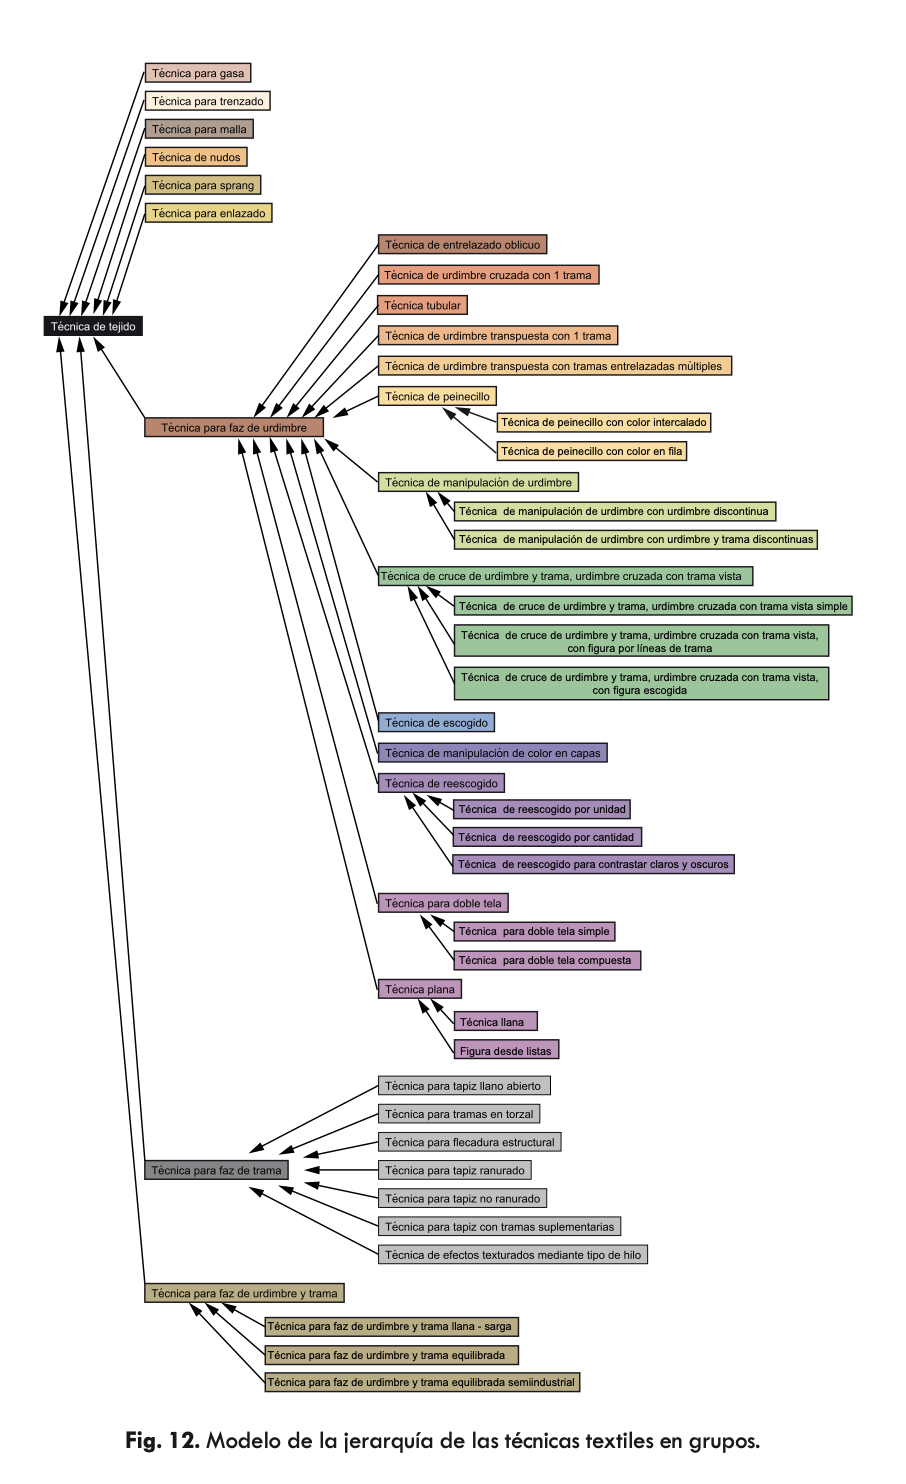
\includegraphics[width=15cm]{images/techniqueArnold32.png}
    \caption[Schéma des techniques présentes dans les Andes]{Schéma des techniques présentes dans les Andes. \\Source : A\textsc{rnold} et E\textsc{spejo}, 2019, p.~32.}
    \label{schemaTechniques}
\end{figure}











\chapter{Préparation des données}
\section{Description des sources et des données}

En première année, j'ai développé un protocole d'apprentissage supervisé à partir de motifs d'un tissu que j'ai à ma disposition. \\

\begin{figure}[!h]
    \centering
    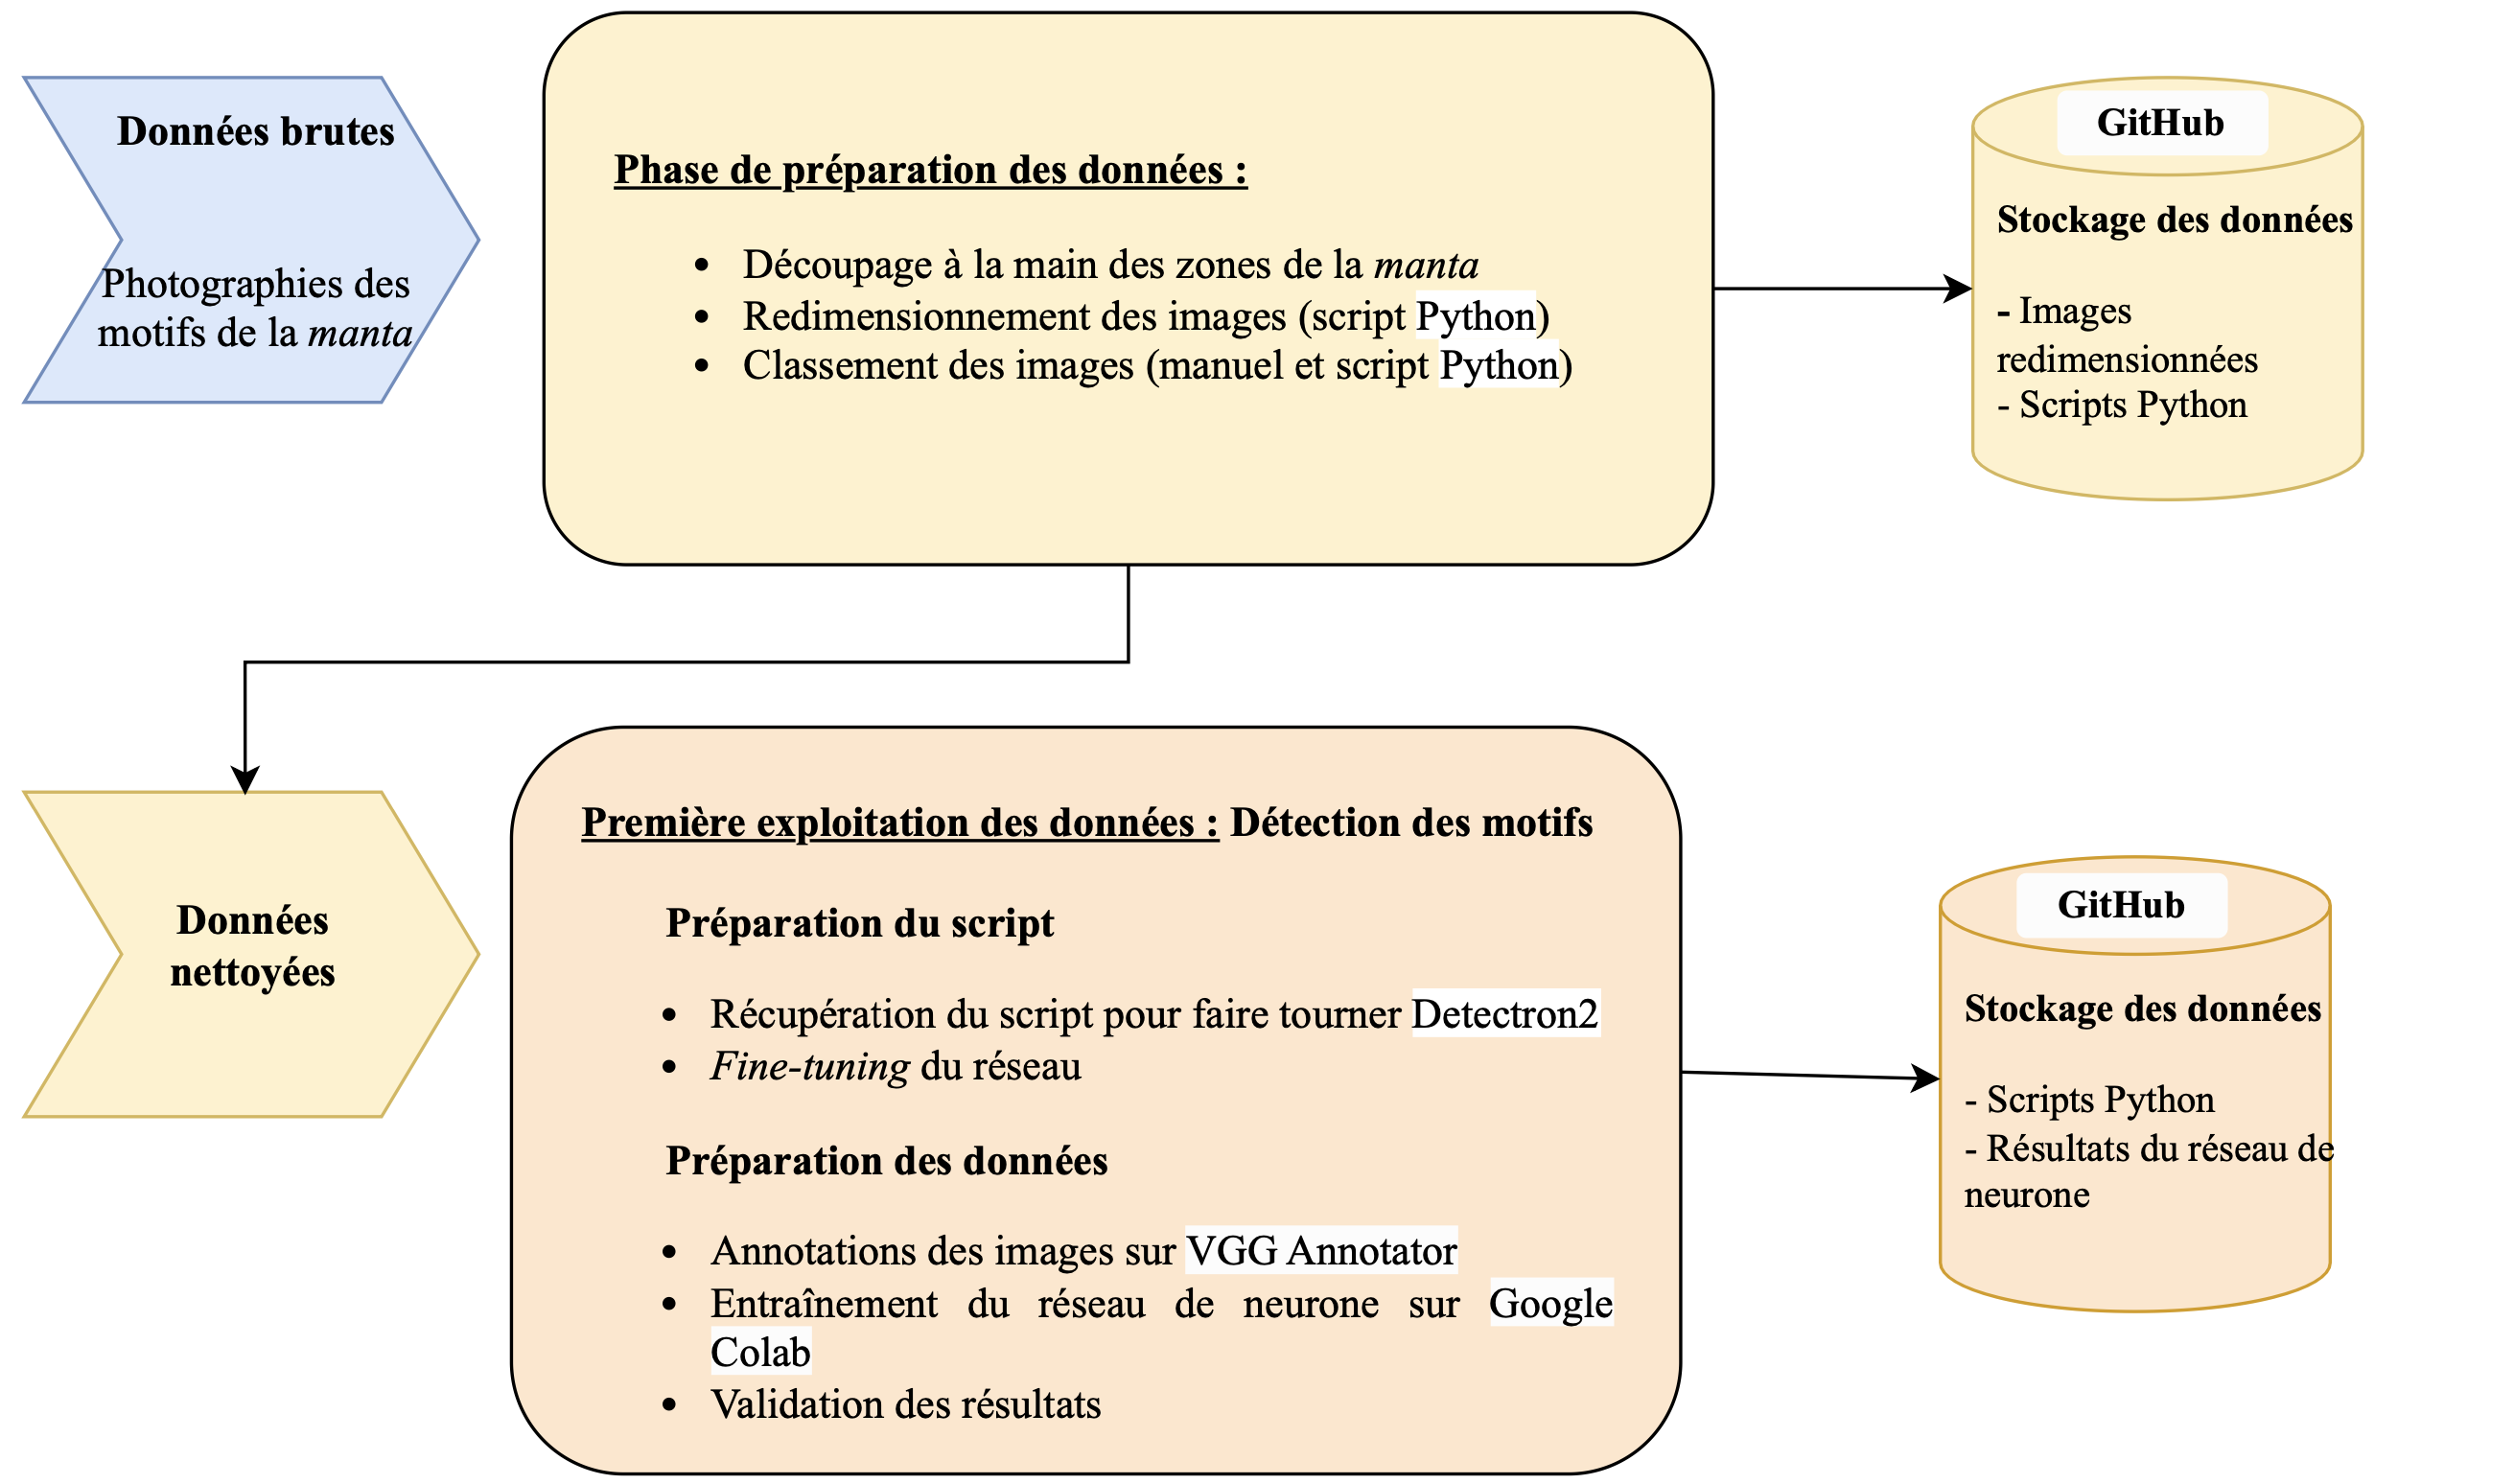
\includegraphics[width=15cm]{images/pipeline.png}
    \caption{Organisation du travail réalisé au cours de la première année de master}
    \label{pipeline}
\end{figure}

\textbf{Description de la source matérielle}

Les images qui composent le corpus de première année sont des photographies d'une \textit{manta} achetée à une tisserande péruvienne au mois de juin 2022. 

Je fais le choix ici de garder le terme \textit{manta} en espagnol puisque son équivalent en français \og mante\fg \:ne me paraît pas correspondre. Les mantes étaient plutôt une partie de l'attirail vestimentaire alors que la \textit{manta} péruvienne se situe entre le châle et le sac. En effet, au Pérou, les \textit{mantas}, ou \textit{lliqlla} en quechua, sont des larges rectangles tissés utilisés comme châles ou pour porter une charge sur le dos. Il est commun de voir une mère porter son enfant en bas âge de cette manière. Les \textit{mantas} font partie des tenues traditionnelles des femmes dans les Andes, et malgré l'évolution des pratiques d'habillement avec l'introduction de vêtements \og mondialisés\fg, elles restent un élément central de la tenue féminine andine, à la fois en milieu rural et en milieu urbain populaire\footnote{Ces observations sont le fruit de mon travail de recherche ethnographique réalisés dans les Andes entre février et août 2022.}. Toutefois, ses caractéristiques ont évolué, de plus en plus de femmes achètent des \textit{mantas} industrielles, réalisées avec des fils en teinture chimique.

\begin{figure}[!h]
    \centering
    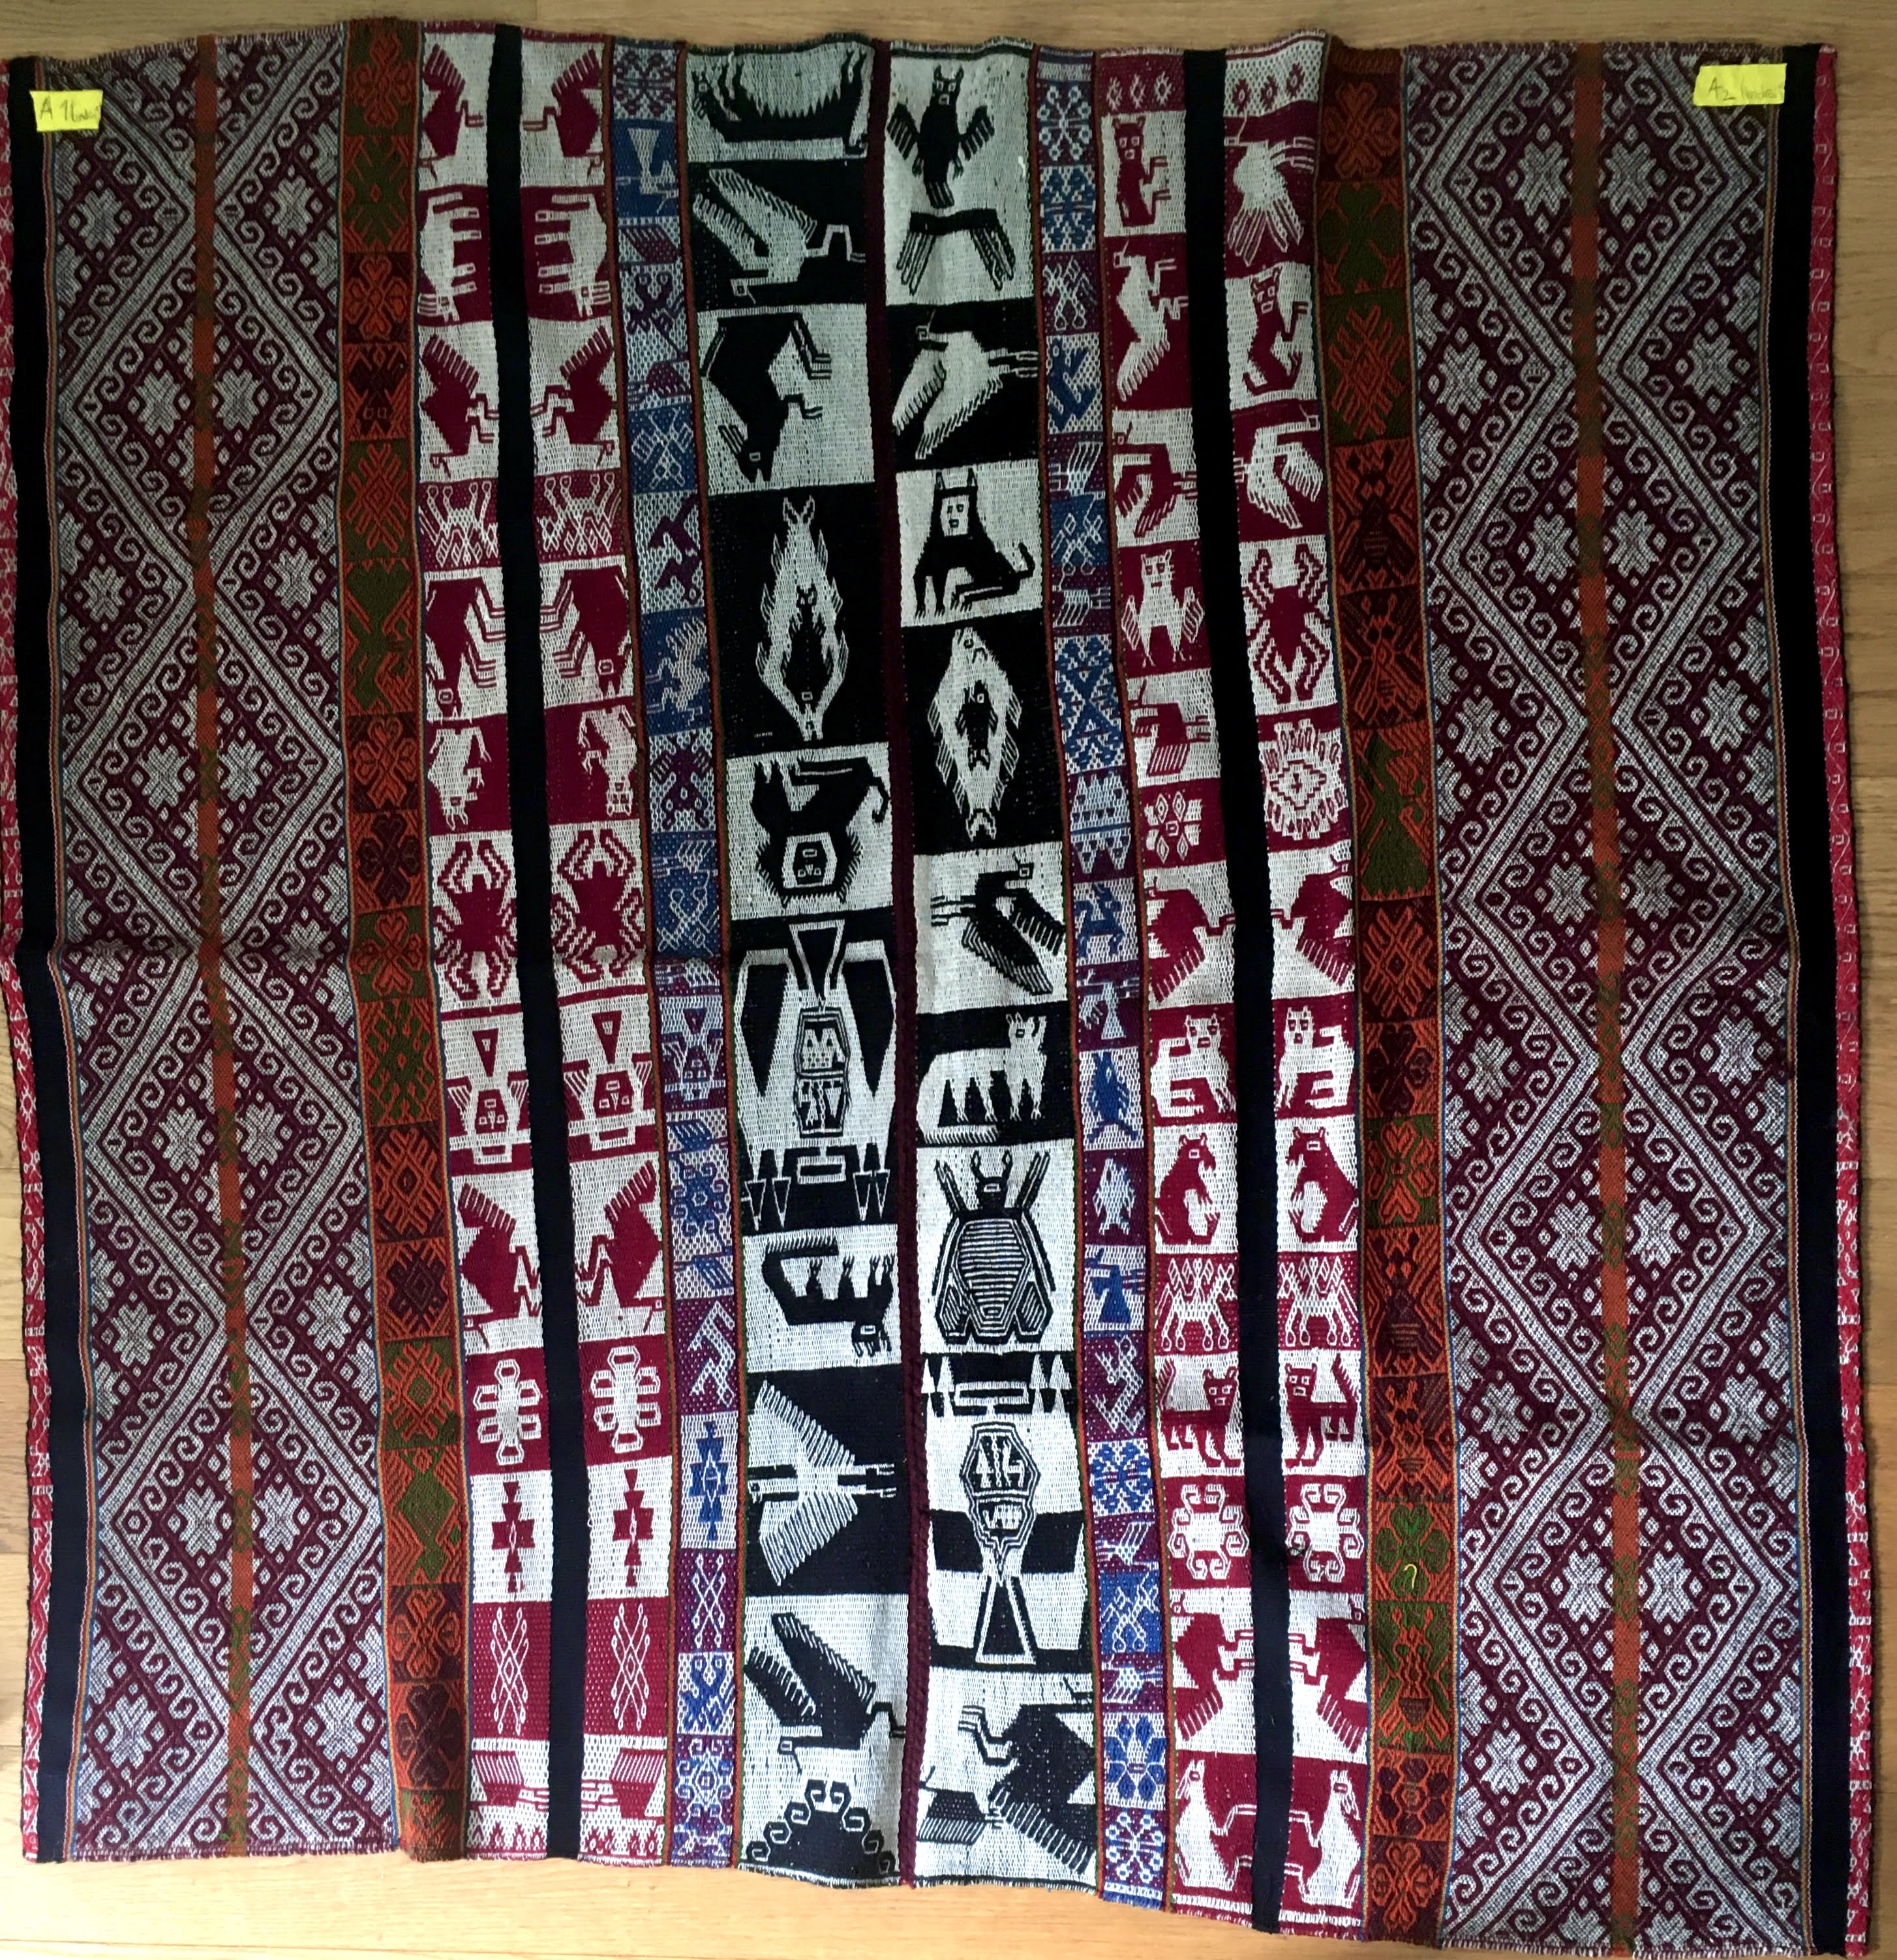
\includegraphics[width=15cm]{images/manta.jpg}
    \caption{Manta étudiée au cours de ce travail}
    \label{manta}
\end{figure}


Pour ma part, il s'agit d'une \textit{manta} réalisée de manière \og traditionnelle \fg \:à Ccachín (Cusco, Andes sud du Pérou). Doña Angelica, la tisserande qui l'a tissée, a acheté les pelotes de fils déjà filés et teints, étapes parfois réalisées en amont du tissage. Elle a donc commencé par ourdir la chaîne --- passage d'un fil d'un piquet à un autre en croisant au centre, de telle sorte à obtenir deux boucles (voir image \ref{ourdissage}) --- déterminant la longueur de la pièce. Enfin, elle a monté la chaîne sur le métier à tisser andin. Ce métier démontable est installé au sol horizontalement ou obliquement sur des piquets en bois (voir image \ref{métierAngelica}).

\begin{figure}[!h]
    \begin{minipage}[c]{.5\linewidth}
            \begin{center}
                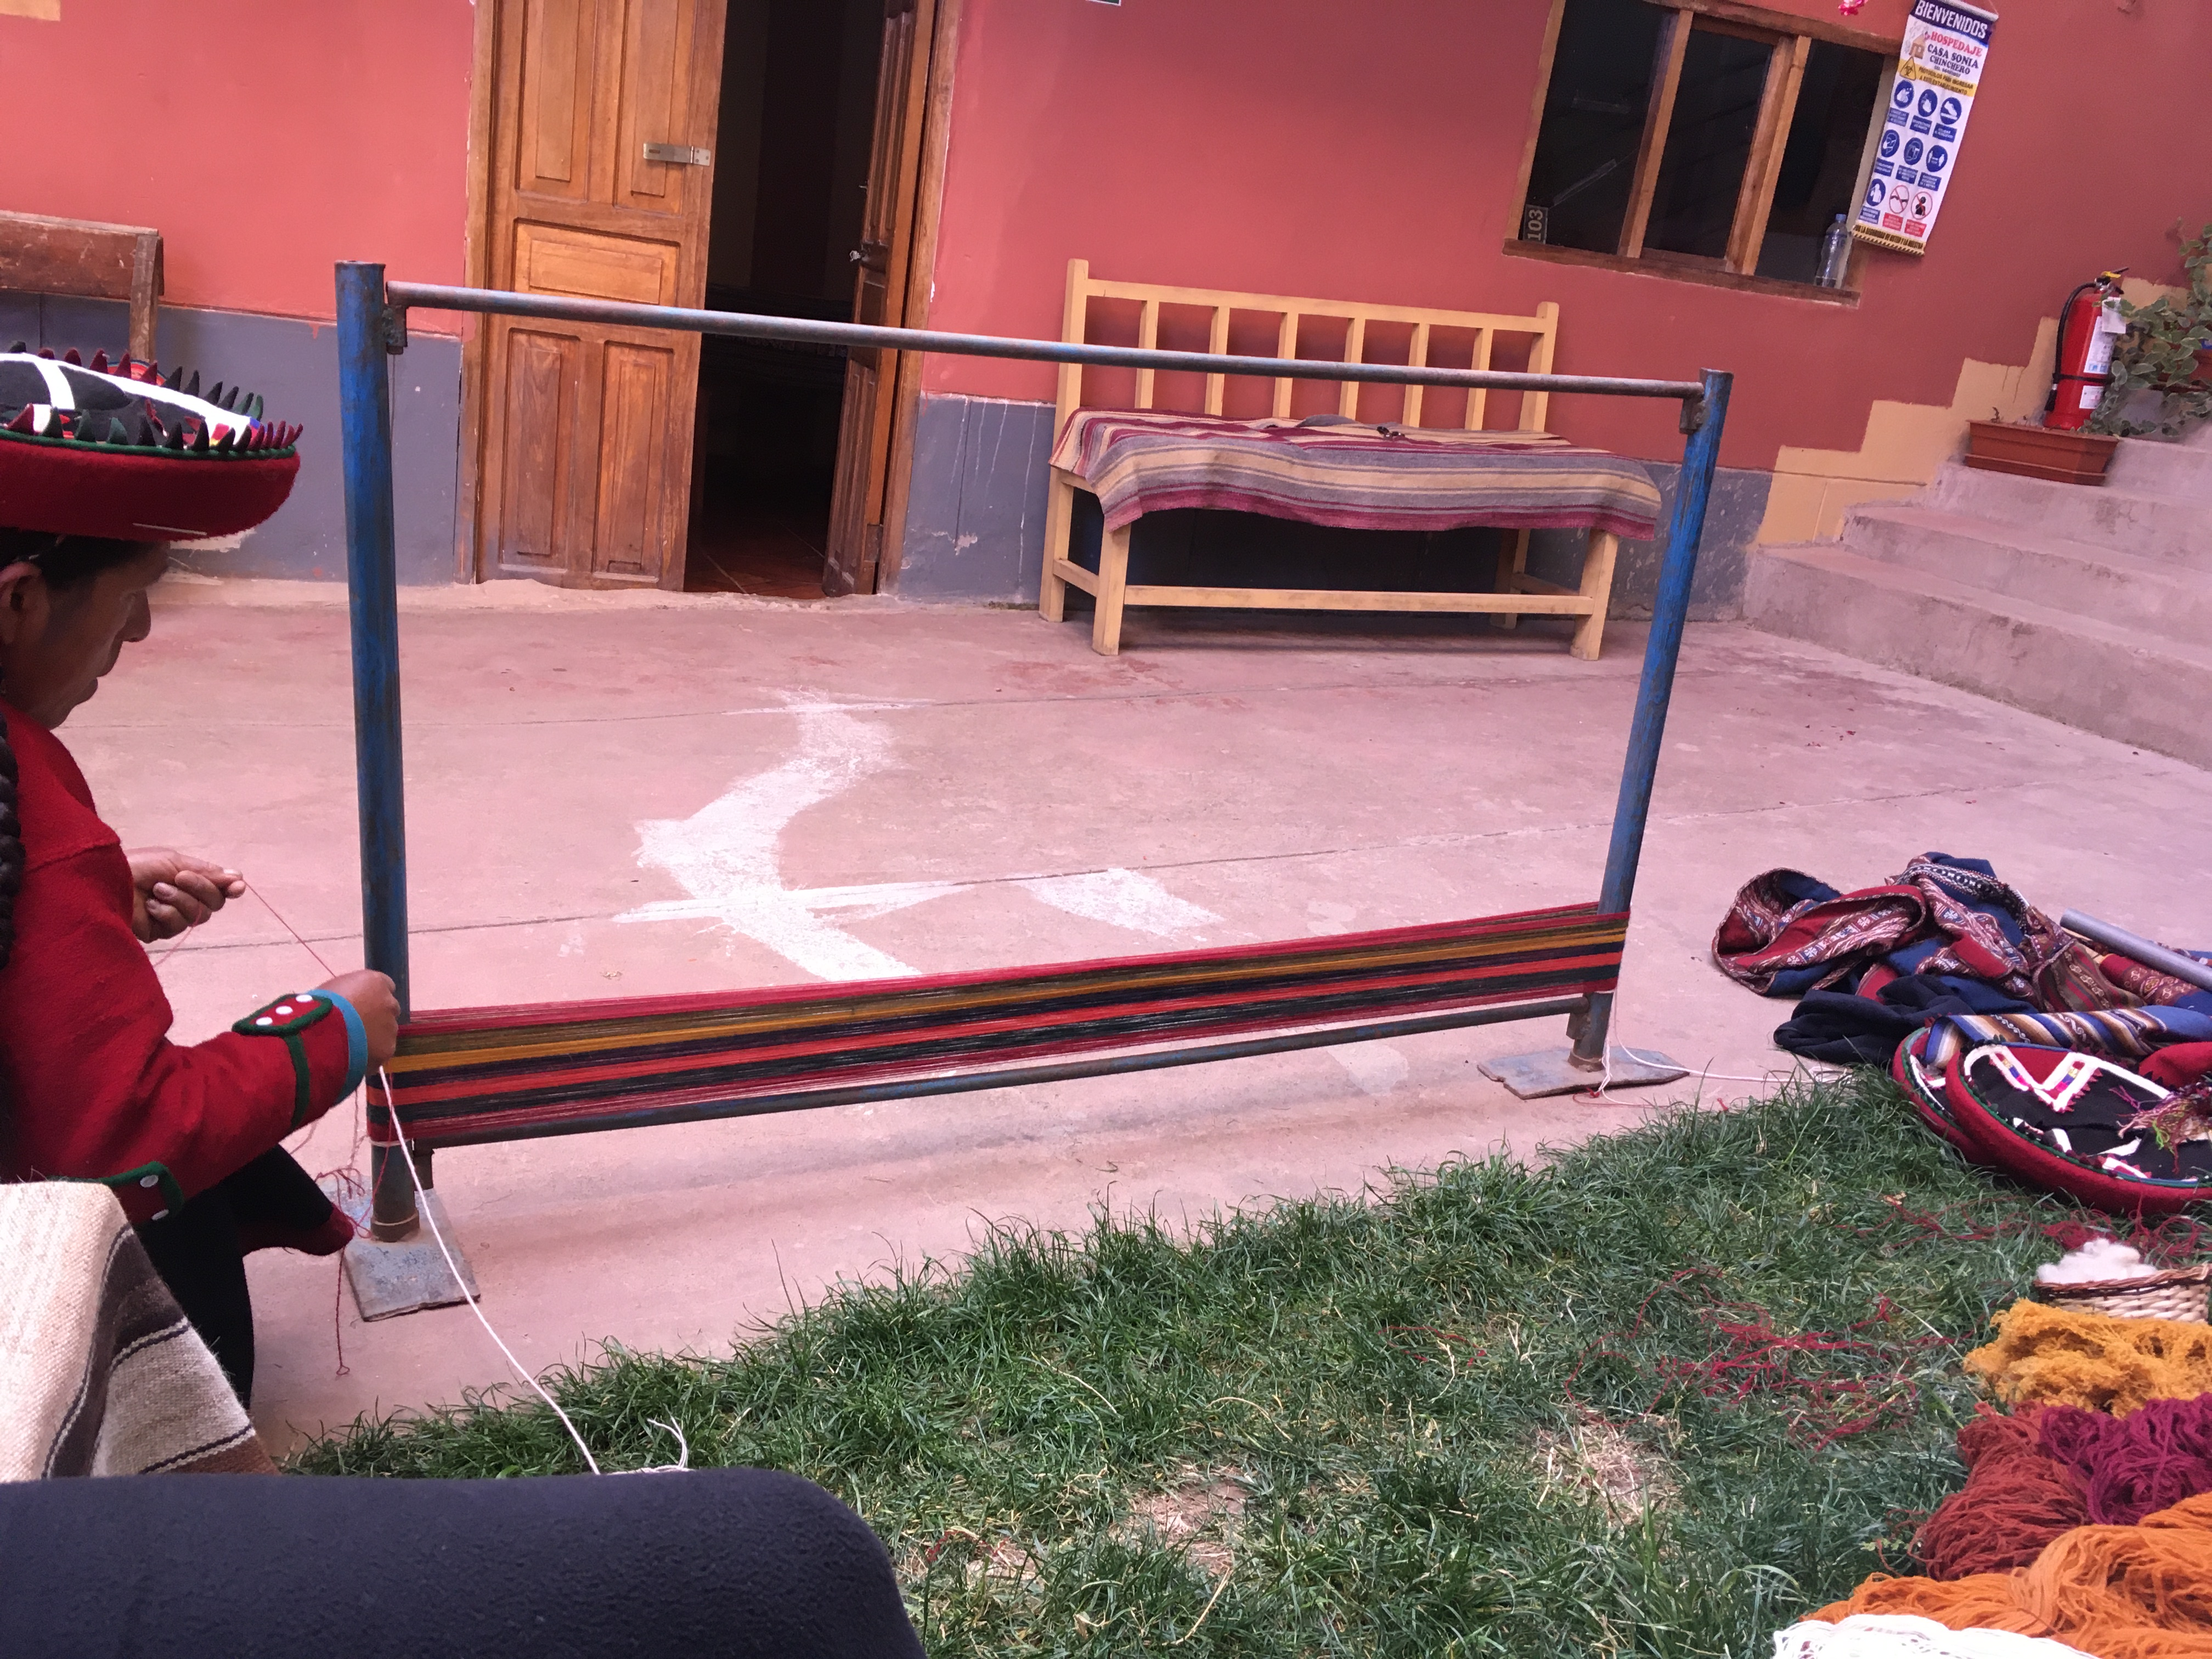
\includegraphics[width=8cm]{images/ourdissage.jpg}
            \caption[Ourdissage d'une chaîne]{Ourdissage d'une chaîne \\ Atelier de Sonia, Chinchero, 13 juillet 2022.}
            \label{ourdissage}
            \end{center}
    \end{minipage}
        \begin{minipage}[c]{.5\linewidth}
            \begin{center}
            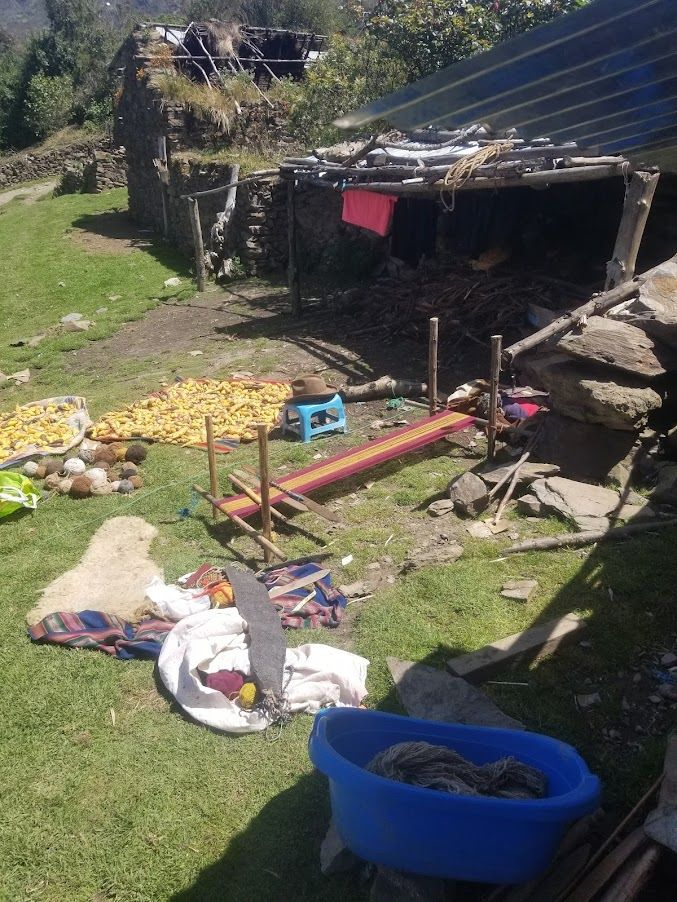
\includegraphics[width=6cm]{images/metierAngelica.jpeg}
            \caption[Métier et chaîne utilisée pour la \textit{manta} étudiée]{Métier et chaîne utilisée pour la \textit{manta} étudiée.\\ Crédit photo : Alice Lhuillier.}
            \label{métierAngelica} 
            \end{center}
    \end{minipage}
\end{figure}

Une fois le métier installé, la tisserande passe la trame dans la chaîne de telle sorte à créer des motifs. Dans notre cas, il s'agit d'un tissage à dominante chaîne ce qui signifie que les fils de chaînes recouvrent la surface du textile, en dissimulant la trame (qui est à l'intérieur du tissu)\footnote{Voir : \cite[p.~1]{centreinternationaldetudedestextilesanciensVocabulaireTechniqueFrancais2020} ou \cite[p.~77]{emeryPrimaryStructuresFabrics1995}}. Dans le cas de cette technique particulière, les fils de chaîne qui sont choisis apparaissent sur la surface et ceux qui ne le sont pas apparaissent sur l'envers du tissu, ainsi les motifs apparaissent en miroir d'un côté et de l'autre de la pièce textile. Pour effectuer la sélection, elle utilise un ensemble de lisses\footnote{Ensemble des mailles tendues côte à côte qui aide à la séparation des fils de chaîne. Source : \cite[p.~29]{centreinternationaldetudedestextilesanciensVocabulaireTechniqueFrancais2020}.}, ses doigts et différents outils. Elle choisit ainsi les fils de chaîne qui apparaîtront sur la surface de la \textit{manta} et ceux qui apparaîtront sur son envers, ainsi que ceux qui ne resteront cachés au sein de la structure textile. Nous retrouvons ici l'idée que le textile ne peux pas être pensé comme un objet en deux dimension puisque techniquement il implique un processus sur trois dimensions. La tisserande avance du bas du métier vers le haut, composant les motifs rangs par rangs (voir image \ref{choix}). Le métier ainsi constitué ne permet pas d'utiliser de navette, la trame est donc passée à la main ce qui génère une contrainte technique : il est difficile de créer une ne pièce plus large que le double de la distance entre le coude et la main. Pour créer des pièces plus larges, comme les \textit{mantas}, il faut alors créer deux pans qui sont cousus pour former un rectangle.

\begin{figure}[!h]
    \begin{minipage}[c]{.5\linewidth}
            \begin{center}
                \includegraphics[width=7cm]{images/lisses.jpg}
                \caption[Lisses]{Utilisation des lisses par Sonia\\ Atelier de Sonia, Chinchero, 13 juillet 2022. \\ Crédit photo : Suzie Robin.}
                \label{lisses}
            \end{center}
    \end{minipage}
    \begin{minipage}[c]{.5\linewidth}
        \begin{center}
            \includegraphics[width=7cm]{images/selectionFils.jpg}
            \caption[Sélection des fils]{Sélection des fils par Sonia\\ Atelier de Sonia, Chinchero, 13 juillet 2022. \\ Crédit photo : Suzie Robin.}
            \label{choix}
        \end{center}
    \end{minipage}
\end{figure}

Par ailleurs, cette technique permet de créer des tissus à quatre lisières, c'est à dire que les quatre côtés du tissu sont fermés et qu'aucun fil n'en sort, les fils coupés étant intégrés dans le tissage. Sophie Desrosiers fait de cette caractéristique un des éléments clés des textiles andins\footcite[par.~8]{desrosiersLogicasTextilesLogicas1997}. Par ailleurs, elle souligne qu'il est encore très mal vu de couper un textile dans les Andes : de nombreuses ethnographies ont relevés que les pièces textiles sont considérées comme des êtres vivants et donc que les couper reviendrait à nuire à leur intégrité\footcite{cerecedaSemiologieTissusAndins1978}. Une autre caractéristique de ces textiles est la volonté d'avoir des pièces équilibrées, la recherche de géométrisation au sein des textiles avec des effets de miroirs est visible sur la plupart des pièces et a été relevée par de nombreux travaux archéologiques et ethnographiques\footnote{Voir notamment : \cite{onealeTextilePeriodsAncient1930}, \cite{cerecedaSemiologieTissusAndins1978} ou \cite{desrosiersLogicasTextilesLogicas1997}.}. Les deux pans d'une \textit{manta} sont donc bien souvent construit de la même manière, alternant des bandes de mêmes couleurs. C'est le cas pour la \textit{manta} que nous allons étudier qui est composée de deux pans différents mais symétriques.

La \textit{manta} étudiée fait 1 mètre 60 par 1 mètre 60. Elle alterne des bandes de \textit{pampa} --- bande unie --- et des bandes de \textit{pallay}\footnote{Terme quechua utilisé pour désigner le dessin qui résulte de la sélection de fils de chaîne que l'on trouve traditionnellement sur les tissages à dominante chaîne réalisés par les femmes dans les communautés.} --- avec des motifs---. Les motifs sont intégrés dans des rectangles dont la couleur du fond alterne. Ce sont des motifs de faune et de flore, des motifs géométriques abstraits et des motifs représentant le visage de Tupac Amaru II\footnote{Révolutionnaire se revendiquant héritier des derniers incas, il mène une rébellion contre les colons espagnols à la fin du \siecle{xviii}. Pour un article reprenant l'historiographie de cette période révolutionnaire : \cite{thomsonCuandoSoloReinasen2010}}.


\begin{figure}[!h]
    \begin{minipage}[c]{.5\linewidth}
            \begin{center}
                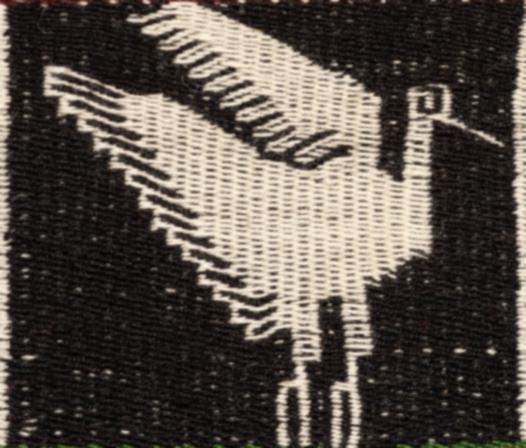
\includegraphics[width=7cm]{images/A2_L02.jpg}
                \caption[Motif noir et blanc]{Motif d'oiseau en noir et blanc}
                \label{nb}
            \end{center}
    \end{minipage}
    \begin{minipage}[c]{.5\linewidth}
        \begin{center}
            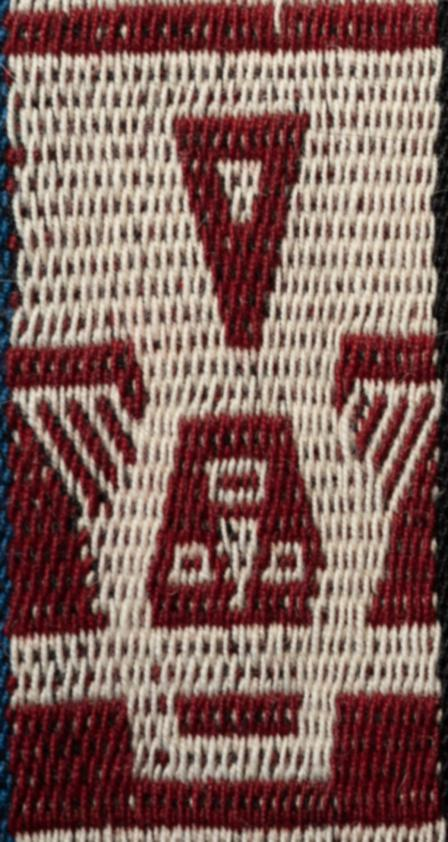
\includegraphics[width=7cm, angle=-180]{images/A1_G08.jpg}
            \caption[Motif rouge et blanc]{Visage de Tupac Amaru en rouge et blanc}
            \label{rb}
        \end{center}
    \end{minipage}
\end{figure}

\begin{figure}[!h]
    \begin{minipage}[c]{.5\linewidth}
            \begin{center}
                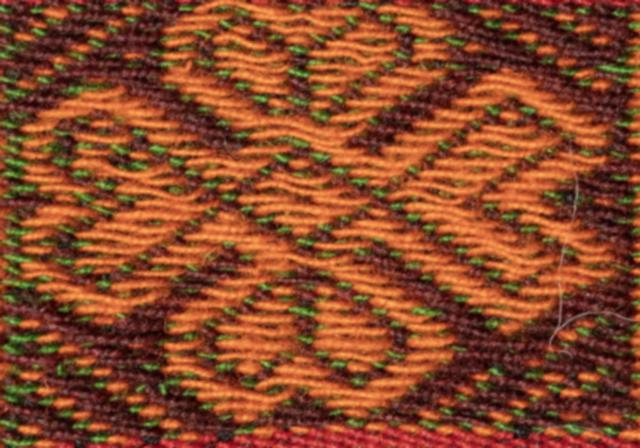
\includegraphics[width=7cm]{images/A1_F07.jpg}
                \caption[Motif orange, marron et vert]{Motif géométrique en orange, marron et vert}
                \label{omv}
            \end{center}
    \end{minipage}
    \begin{minipage}[c]{.5\linewidth}
        \begin{center}
            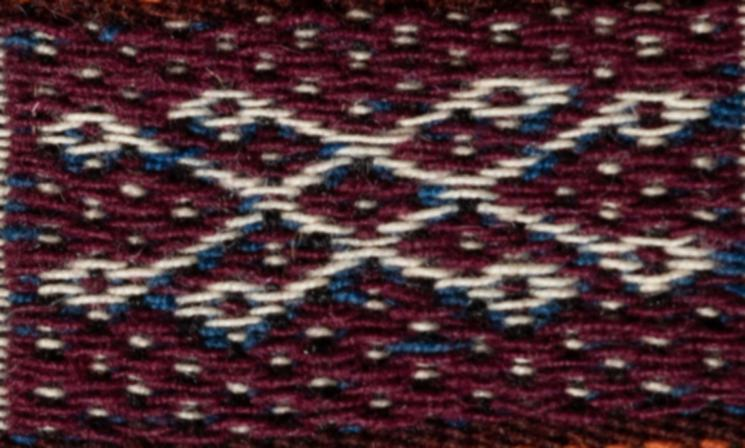
\includegraphics[width=7cm]{images/A1_I13.jpg}
            \caption[Motif blanc, bleu et violet]{Motif géométrique en blanc, bleu et violet}
            \label{bbv}
        \end{center}
    \end{minipage}
\end{figure}

Les quatre type de motifs sont à dominante chaîne avec l'utilisation des chaînes complémentaire. D'après la classification d'Irene Emery, les chaînes complémentaires sont quand \og deux ou plusieurs ensembles d’éléments [ici la chaîne] ont la même direction dans un tissu et sont co-égaux dans la structure du tissu\fg\footnote{\cite[p.~150]{emeryPrimaryStructuresFabrics1995}. ''\textit{when two or more sets of elements have the same direction in a fabric and are co-equal in the fabric structure}''}. C'est le recours à cette technique qui crée cet effet de miroir et implique que les motifs qui sont sur l'endroit du tissu apparaissent de la couleur de la seconde chaîne sur l'envers du tissu. C'est l'alternance de l'apparition des chaînes qui crée différents aplats de couleur. Ainsi, ce qui distingue les techniques qui apparaissant dans la \textit{manta} ce sont le nombre de chaînes complémentaire par bande. Pour les motifs noir et blanc ou blanc et rouge, seules deux chaînes complémentaires sont nécessaires. Pour les motifs blanc, bleu et violet ou orange, marron et vert, trois chaînes complémentaires sont nécessaires. 

Le motif de Tupac Amaru II est particulièrement intéressant car c'est un visage humain géométrisé dont la présence permet d'attester le lieu d'origine de la pièce. En effet, ce motif est typique de la région de Calca où se trouve le village de Ccachín. Ce thème est central dans l'histoire nationale péruvienne et des motifs le représentant ont donc intégré les tissages. Les représentations tissées les plus fréquentes sont le visage de Tupac Amaru, avec son chapeau caractéristique, et la croix représentant la scène de l'écartèlement. \\


\textbf{Description de la source numérique}

Pour travailler à partir des images de la \textit{manta}, nous avons photographié chaque motif avec un appareil photographique \textsc{sony ilce-}\small9\normalsize, soit 272 photographies de 272 motifs. Nous avons donc laissé de côté les bandes unies ainsi que les deux bandes sur les bords. Nous nous sommes concentrés sur les rectangles qui contiennent un motif. Par ailleurs, nous avons fait en sorte d'avoir un éclairage neutre et régulier afin d'obtenir les couleurs numériques les plus proches possibles de la réalité des fils.

\begin{table}[!h]
    \centering
    \begin{tabular}{|c|c|}
        \hline
        Dimension & Résolution \\ \hline 
        6000 x 4000 & 300 x 300 \\ \hline
    \end{tabular}
    \caption{Caractéristiques techniques des photographies initiales.}
    \label{tab:tableau1}
\end{table}

Les images sont donc de très grande qualité et permettent d'obtenir le détail des fils. Toutefois, elles sont lourdes à utiliser. Par ailleurs, les quatre catégories présentes sur la \textit{manta} ne sont pas équilibrées. Les motifs noirs et blanc étant plus grands, ils sont moins nombreux. À l'inverse, les bandes de motifs rouge et blanc sont plus nombreuses ce qui explique le nombre plus élevé pour ces motifs.

\begin{table}[!h]
    \centering
    \begin{tabular}{|c|c|c|}
        \hline
        \cellcolor{blue!20}\textbf{Type de motif }& \cellcolor{blue!20} \textbf{Nombre d'images} & \cellcolor{blue!20} \textbf{Pourcentage du corpus d'images} \\ \hline \hline
        Motifs noir et blanc & 36 & 13\% \\ \hline
        Motifs rouge et blanc & 110 & 40\% \\ \hline
        Motifs orange, marron et vert  & 62 & 23\% \\ \hline
        Motifs blanc, bleu et violet  & 64 & 24\% \\ \hline
        \textbf{Total} & \textbf{272} & \textbf{100\%} \\ \hline
        
    \end{tabular}
    \caption{Caractéristiques du corpus d'images final.}
    \label{tab:tableau2}
\end{table}

\section{Pré-traitement des images}

\textbf{Découpage des images}

Avant d'exploiter les images, il faut les mettre en forme pour qu'elles puissent être traitées et fournir de bons résultats. Pour cela, nous avons détouré les rectangles pour obtenir une image contenant un unique motif. Cette étape a été faite à la main, notamment sur le logiciel Photoshop. Cela a aussi permis de vérifier que nous avions des photographies de bonne qualité pour tous les motifs. Pour cela, nous avons créé une modélisation basique de la \textit{manta} sur Excel (voir le document \og model\_manta.xlsx\fg \:dans le GitHub). Cela nous a aussi permis d'attribuer aux images un identifiant unique : une première lettre indique le pan (A ou B) associée à un chiffre pour la face (1 ou 2) puis, séparé pas un tiret bas, une lettre indique la bande (de A à T) et un chiffre le numéro du motif (de 1 à 17). Ainsi, le motif A1\_G06 se trouve sur l'avant du premier pan (indiqué sur l'objet physique) et est le 6\textsuperscript{ème} motif de la 7\textsuperscript{ème} bande. Nous avons donc fait en sorte de renommer les images suivant cette codification afin de pouvoir associer les motifs à leurs caractéristiques physiques. Du fait de la symétrie entre les deux plans, des motifs comportant la même lettre de colonne ont la même technique. Cela permet aussi de détecter l'endroit et l'envers d'un motif dont seul le premier numéro change (1 ou 2). \\

\textbf{Redimensionnement des images}

Le redimensionnement des images a été fait de telle sorte que la taille des images ne dépasse pas 448 pixels. Le redimensionnement permet à la fois d'entraîner plus rapidement le modèle et de limiter la taille du \textit{padding} autour de l'image. Le \textit{padding} est l'espace ajouté par le réseau de neurone autour des images au moment de l'entraînement pour que la dimension totale de l'image corresponde à celle des autres images, sans déformer leur contenu. Pour cela, nous avons suivi la démarche de Clermont et al. (2020)\footcite{clermontAssessingSemanticSimilarity2020} et nous avons fait en sorte que la plus grande dimension des images (largeur ou hauteur) soit d'exactement 448 pixels\footnote{Voir le module \og rescaleImages.py\fg \:dans le GitHub, une partie du script est issue du répertoire \og silknow\_image\_classification \fg \:du GitHub de \textsc{silknow}, \url{https://github.com/silknow/image-classification} (consulté le 10 juin 2023). Ce module doit être lancé dans le même dossier que le dossier \og \\img\_unscaled\fg \:où se trouve les images.}. Nous nous réservons la possibilité de faire varier la taille des images en fonction des résultats finaux du réseau.

\section{Organisation des images}

La seconde partie de la préparation des images portait sur l'organisation des images afin d'obtenir le corpus d'images le plus équilibré possible.

Le recours à la feuille Excel permettant de nommer les images a permis d'accélérer le processus d'organisation. Par ailleurs, nous avons utilisé un court script permettant de récupérer les noms des images dans un document texte afin d'affiner cette vérification\footnote{Voir le script \og noms\_images\_txt.py\fg.}.

La \textit{manta} est composée de quatre catégories différentes, nous avons donc fait en sorte d'obtenir des données d'entraînement, de validation et de test les plus équilibrées possible. Les données d'entraînement sont les données à partir desquelles le réseau de neurones \og apprend \fg \:à détecter l'information que l'on recherche. Les données de validation permettent de vérifier la qualité de l'entraînement et les données test permettent de venir affiner les paramètres du modèle.

Cependant, nous savons déjà que nous ne disposons pas du même nombre d'images pour chaque catégorie déterminée (voir tableau \ref{tab:tableau2}). Pour pallier cela, nous avons réparti les images redimensionnées entre quatre dossiers, chacun correspondant à une technique (en distinguant les motifs noir et blanc des motifs rouge et blanc, la couleur pouvant avoir une influence sur l'entraînement), afin d'obtenir des échantillons représentatifs du corpus. Ensuite, nous avons utilisé un script de division du \textit{dataset} issu de la librairie Python split-folders avec un ratio de 80\% de données d'entraînement, 10\% de données de validation et 10\% de données test. Nous avons ainsi dans chacune de ces catégories un ensemble de motifs de chaque technique ou couleur. 

\begin{table}[!h]
    \centering
    \begin{tabular}{|c|c|c|c|}
        \hline
        & \cellcolor{blue!20}\textbf{Données entraînement}& \cellcolor{blue!20} \textbf{Données validation} & \cellcolor{blue!20} \textbf{Données test} \\ \hline \hline
         Pourcentage & 80\% & 10\% & 10\% \\ \hline
         Nombre d'images & 216 & 26 & 30 \\ \hline
        
    \end{tabular}
    \caption{Répartition des données.}
    \label{tab:trainTest}
\end{table}



\chapter{Exploitation des données}
\section{Un réseau de neurones pour détecter les motifs ? }

Pour pouvoir analyser les évolutions spatiales et temporelles des pièces textiles, notamment à partir de leurs motifs, il faut développer un outil qui permettrait de détecter automatiquement et d'extraire ces motifs. Pour cela, les réseaux de neurones convolutifs (CNN) semblent être le meilleur outil puisqu'ils ont pour but d'extraire des informations à partir d'une image. 

\begin{figure}[!h]
    \centering
    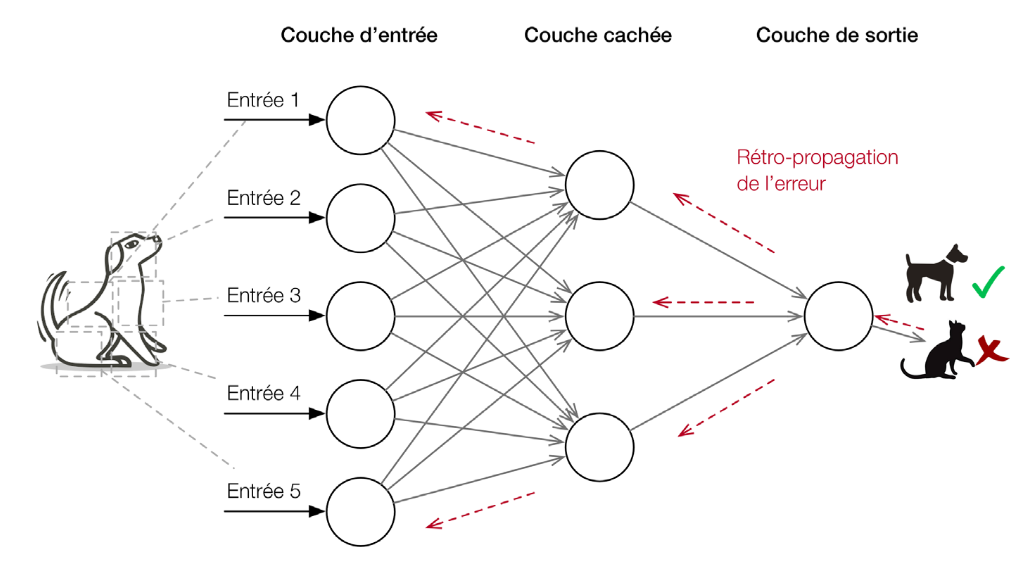
\includegraphics[width=12cm]{images/resSimple_CardonP199.png}
    \caption[Structure simple d'un réseau de neurones]{Structure simple d'un réseau de neurones \\ Source : C\textsc{ardon} et al., 2018, p.~199}
    \label{resSimple}
\end{figure}

En 1943, Warren S. McCulloch et Walter Pitts proposent le premier modèle dans le domaine de la neurophysiologie qui est associé au concept d'apprentissage\footcite{mccullochLogicalCalculusIdeas1943}. C'est un modèle au sein duquel \og le neurone prend des variables en entrées, y applique un poids pour produire une somme qui, si elle dépasse un certain seuil, déclenche l'activation du neurone\footcite{cardonRevancheNeuronesInvention2018}\fg. Il sert de référence à une grande partie du domaine de l'intelligence artificielle pendant plusieurs décennies. Dans les années 2010, la publication d'Alex Krizhevsky et Geoffrey Hinton, descendante de ce premier modèle, modifie profondément le domaine de la classification d'images\footcite{krizhevskyLearningMultipleLayers2009}. Ils proposent de classifier un ensemble de plus d'un million d'image grâce à un réseau de neurones \og convolutif\fg. Les réseaux convolutifs sont composés d'un ensemble de couches dont \og les couches additionnelles de neurones permettent d'apprendre des fonctions non linéaires. L'algorithme fonctionne en prenant la dérivée de la fonction de perte du réseau et en \textquotedblleft propage'' l'erreur pour corriger les coefficients dans les couches basses du réseau\footcite[p.~198]{cardonRevancheNeuronesInvention2018}.\fg

\begin{figure}[!h]
    \centering
    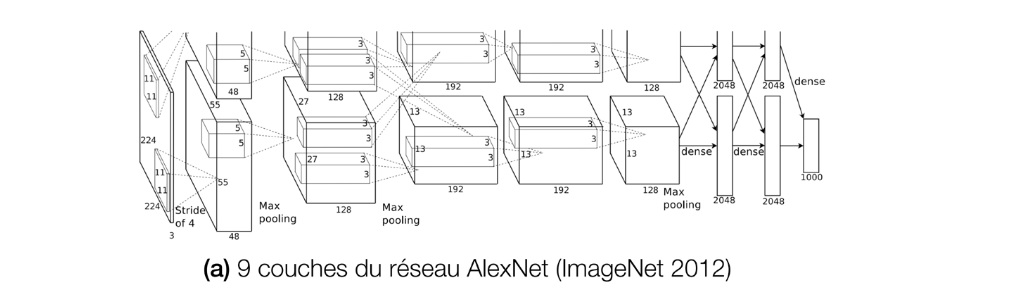
\includegraphics[width=15cm]{images/structureAlexNetCNN_CardonP211.png}
    \caption[Structure d'un réseau de neurones de type \og convolutif\fg]{Structure d'un réseau de neurones de type \og convolutif\fg \\ Source : C\textsc{ardon} et al., 2018, p.~211}
    \label{CNN} 
\end{figure}

Dans notre cas particulier, nous avons décidé d'utiliser Detectron2, le réseau convolutif proposé par Facebook. Il succède à Detectron et Mask R-CNN.
Pour des raisons techniques, notamment pour gagner en efficacité, nous avons utilisé ce modèle au sein de \textit{Google Colaboratory} qui donne accès à des processeurs graphiques qui facilitent les calculs à partir d'images\footnote{Le notebook contenant le code, nommé \og Detectron2\_liseCOLAB.ipynb\fg, est donc adapté à une installation dans \textit{Google Colaboratory}. Voir la documentation de Detectron2 : \url{https://detectron2.readthedocs.io/en/latest/}}. \\

\textbf{Annotations des images}

Pour entraîner le modèle Detectron2, il faut lui fournir des images annotées c'est-à-dire des images pour lesquelles le motif est détouré, ce qui permet au réseau \og d'apprendre \fg \:à reconnaître les motifs. Ces zones, qu'on nomme régions d'intérêt (\textit{region of interest} ou RoI), seront traitées par les couches du réseau qui prédit ensuite si une région d'intérêt est présente dans une image ou non. 

Cette étape d'annotation est l'étape la plus fastidieuse du processus puisqu'elle est très chronophage, d'autant plus que les motifs sont constitués d'un ensemble de petits détails. Cette annotation s'est faite à l'aide de l'outil VGG Image Annotator (VIA) proposé par l'Université d'Oxford\footnote{Voir \url{https://www.robots.ox.ac.uk/~vgg/}, consulté le 20 mai 2023.}. Après avoir annoté les images, il est possible de récupérer les coordonnées des éléments annotés dans les images en format COCO json, format qui est requis par Detectron2 pour entraîner le modèle. Grâce à la fonctionnalité \og polygones \fg \:de VIA, il est possible de détourer très précisément les images. Les annotations reposent en grande partie sur la vision humaine, ainsi la couleur n'est pas le seul déterminant de la distinction entre fond et motif. Par ailleurs, le textile contient des défauts ou bien des irrégularités que l'annotation permet de mettre de côté (comme sur l'image \ref{VIAdefaut} pour laquelle la chaîne rouge ressort alors qu'elle ne compose pas le motif). Nous pouvons aussi relever sur l'image \ref{VIAambi} la présence de fils flottants, c'est-à-dire des fils de chaîne qui restent à la surface sur plusieurs passages de trame. De par leur filage manuel, ces fils ne restent pas rectilignes et ondulent à la surface ce qui peut créer des irrégularités dans l'image.

\begin{figure}[!h]
    \begin{minipage}[c]{.5\linewidth}
            \begin{center}
                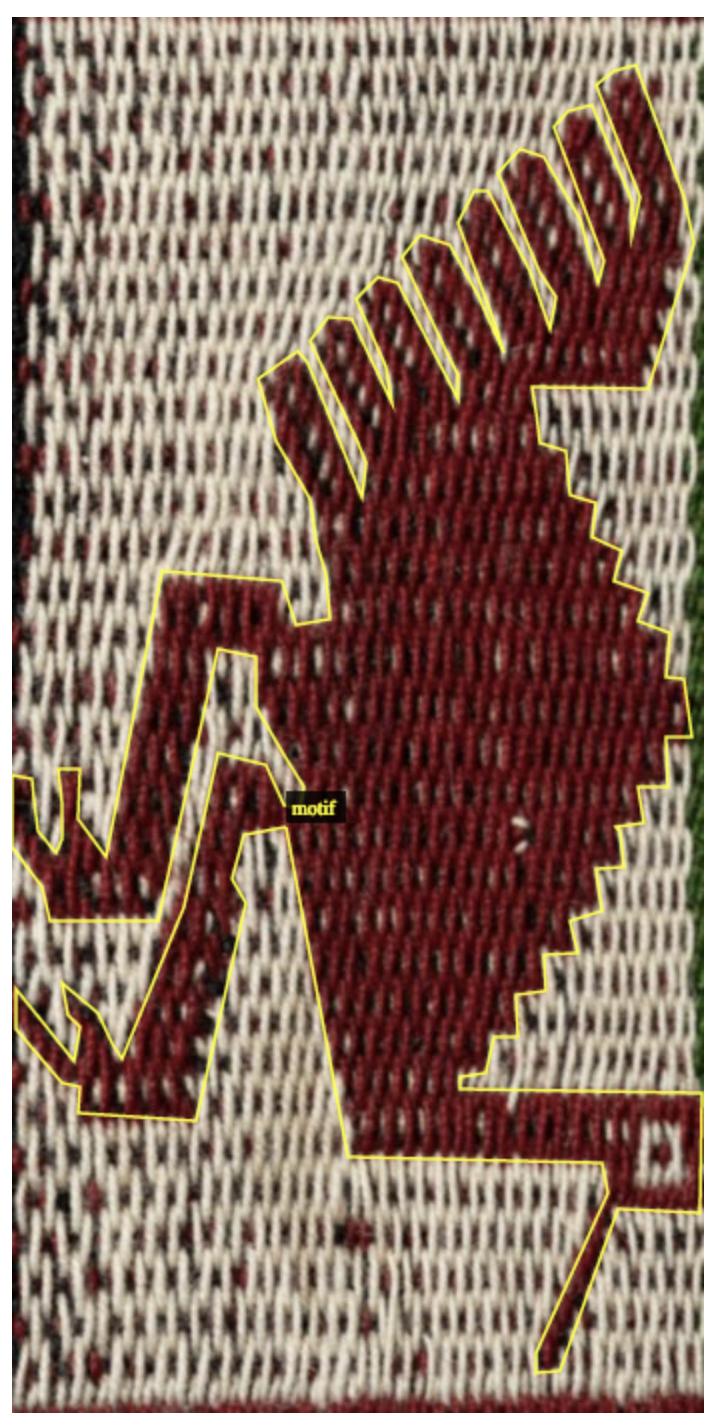
\includegraphics[width=4cm]{images/imageVIA.png}
                \caption[Annotation de motif]{Annotation de motif sur le \\logiciel VIA.}
                \label{VIA}
            \end{center}
    \end{minipage}
    \begin{minipage}[c]{.5\linewidth}
        \begin{center}
            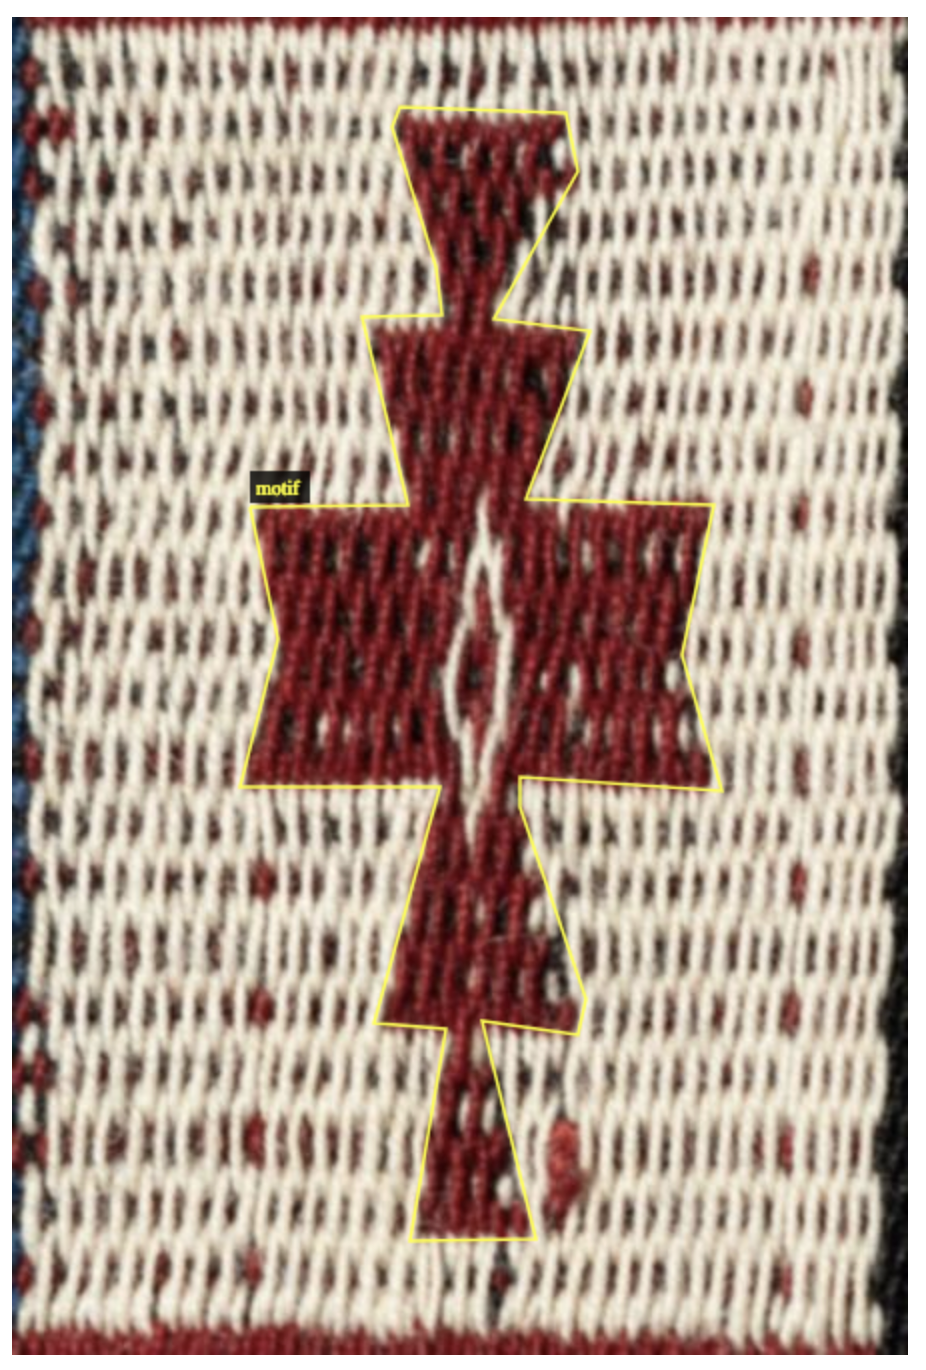
\includegraphics[width=6cm]{images/defautAnnotation.png}
            \caption{Annotation de motifs avec \\ défaut dans le tissu}
            \label{VIAdefaut}
        \end{center}
    \end{minipage}
\end{figure}

\begin{figure}[!h]
    \begin{minipage}[c]{.5\linewidth}
            \begin{center}
                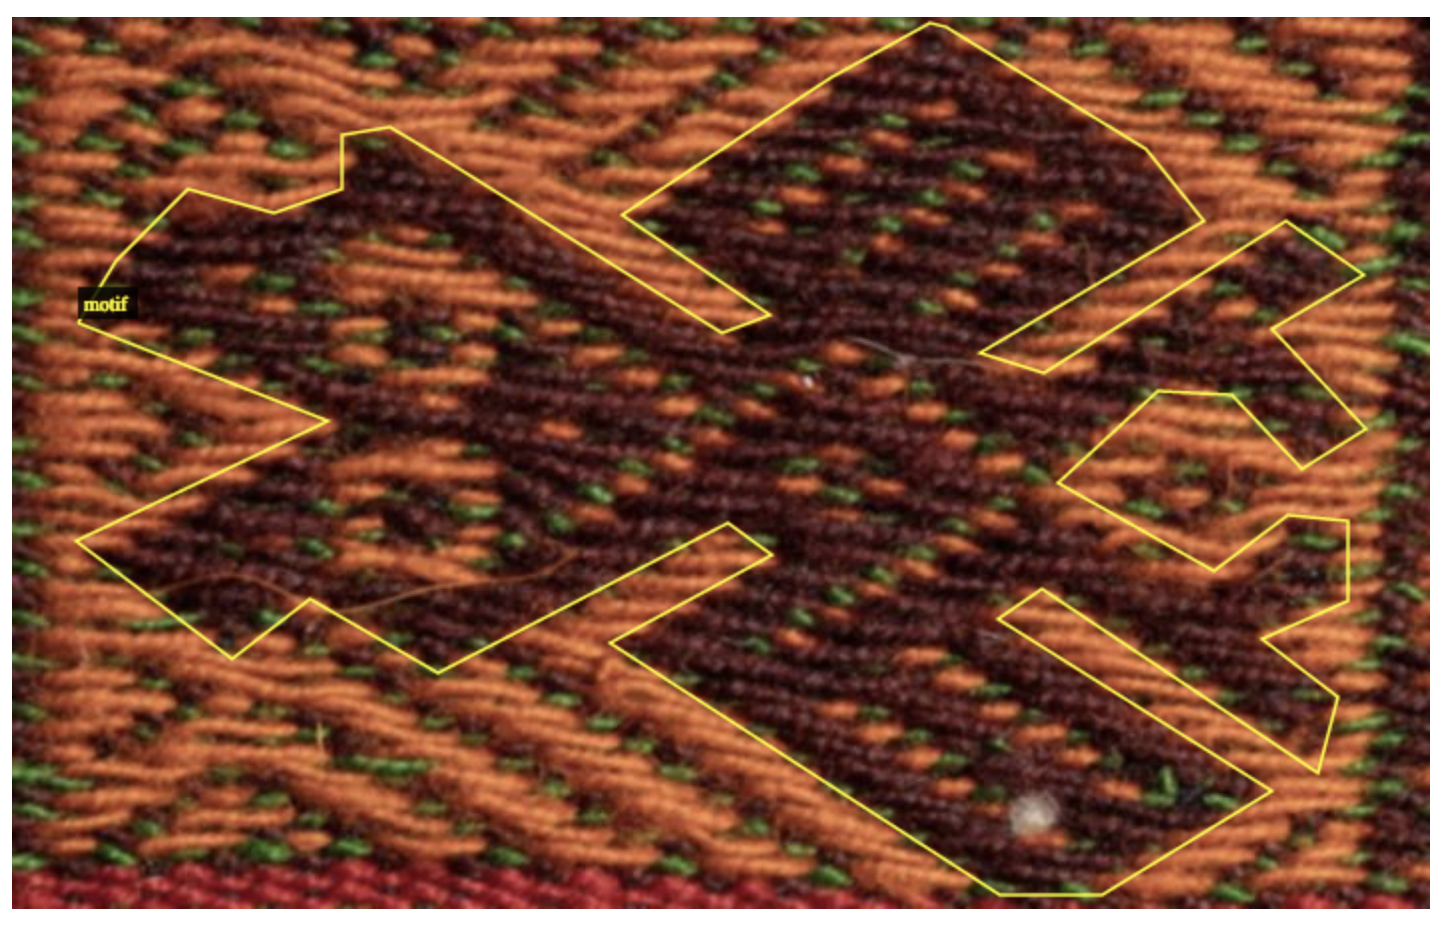
\includegraphics[width=6cm]{images/annotations.png}
                \caption[Annotation de motif]{Annotation de motif sur le \\ logiciel VIA.}
                \label{VIAchouette}
            \end{center}
    \end{minipage}
    \begin{minipage}[c]{.5\linewidth}
        \begin{center}
            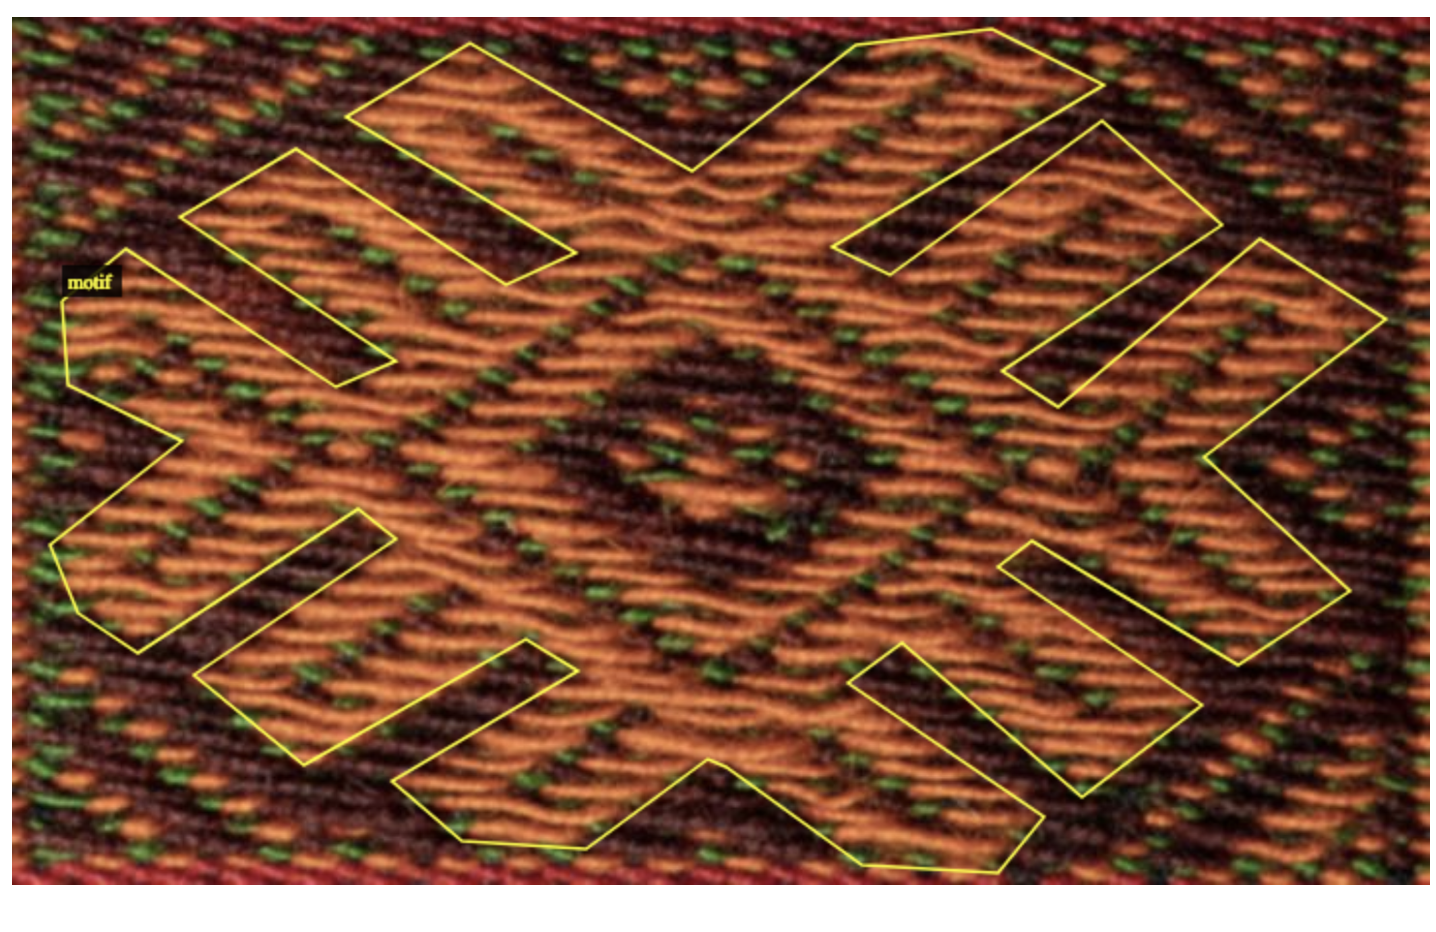
\includegraphics[width=6cm]{images/ambiguAnnotations.png}
            \caption[Annotation de motif]{Annotation de motif sur le \\logiciel VIA.}
            \label{VIAambi}
        \end{center}
    \end{minipage}
\end{figure}

Par ailleurs, au début du projet nous avions pensé faire détecter les différentes chaînes du textile, mais c'est plutôt l'entrecroisement des chaînes qui est intéressant puisqu'il forme le motif. Ainsi pour la chouette (image \ref{VIAchouette}), la chaîne qui compose le fond (orange) est aussi celle qui forme les yeux de l'oiseau et donc fait partie intégrante du motif. Au moment de l'annotation la question du remplissage s'est posée. Pour certaines images en effet nous avons détouré le motif, le considérant rempli alors même que la présence d'une deuxième chaîne en son sein pourrait laisser penser que le motif n'est pas plein (comme sur l'image \ref{VIAambi}). \\

\textbf{Code utilisé}

Dans un premier temps, nous installons Detectron2 ainsi que toutes les librairies nécessaires dans le \textit{notebook} où nous travaillons pour la partie informatique. 

La première étape du code consiste à vérifier la lisibilité des images et des annotations par les librairies Detectron2. Comme nous pouvons le voir sur l'image ci-dessous, cette étape est fonctionnelle, les motifs sont bien détourés et leurs annotations sont lisibles.

\begin{figure}[!h]
    \centering
    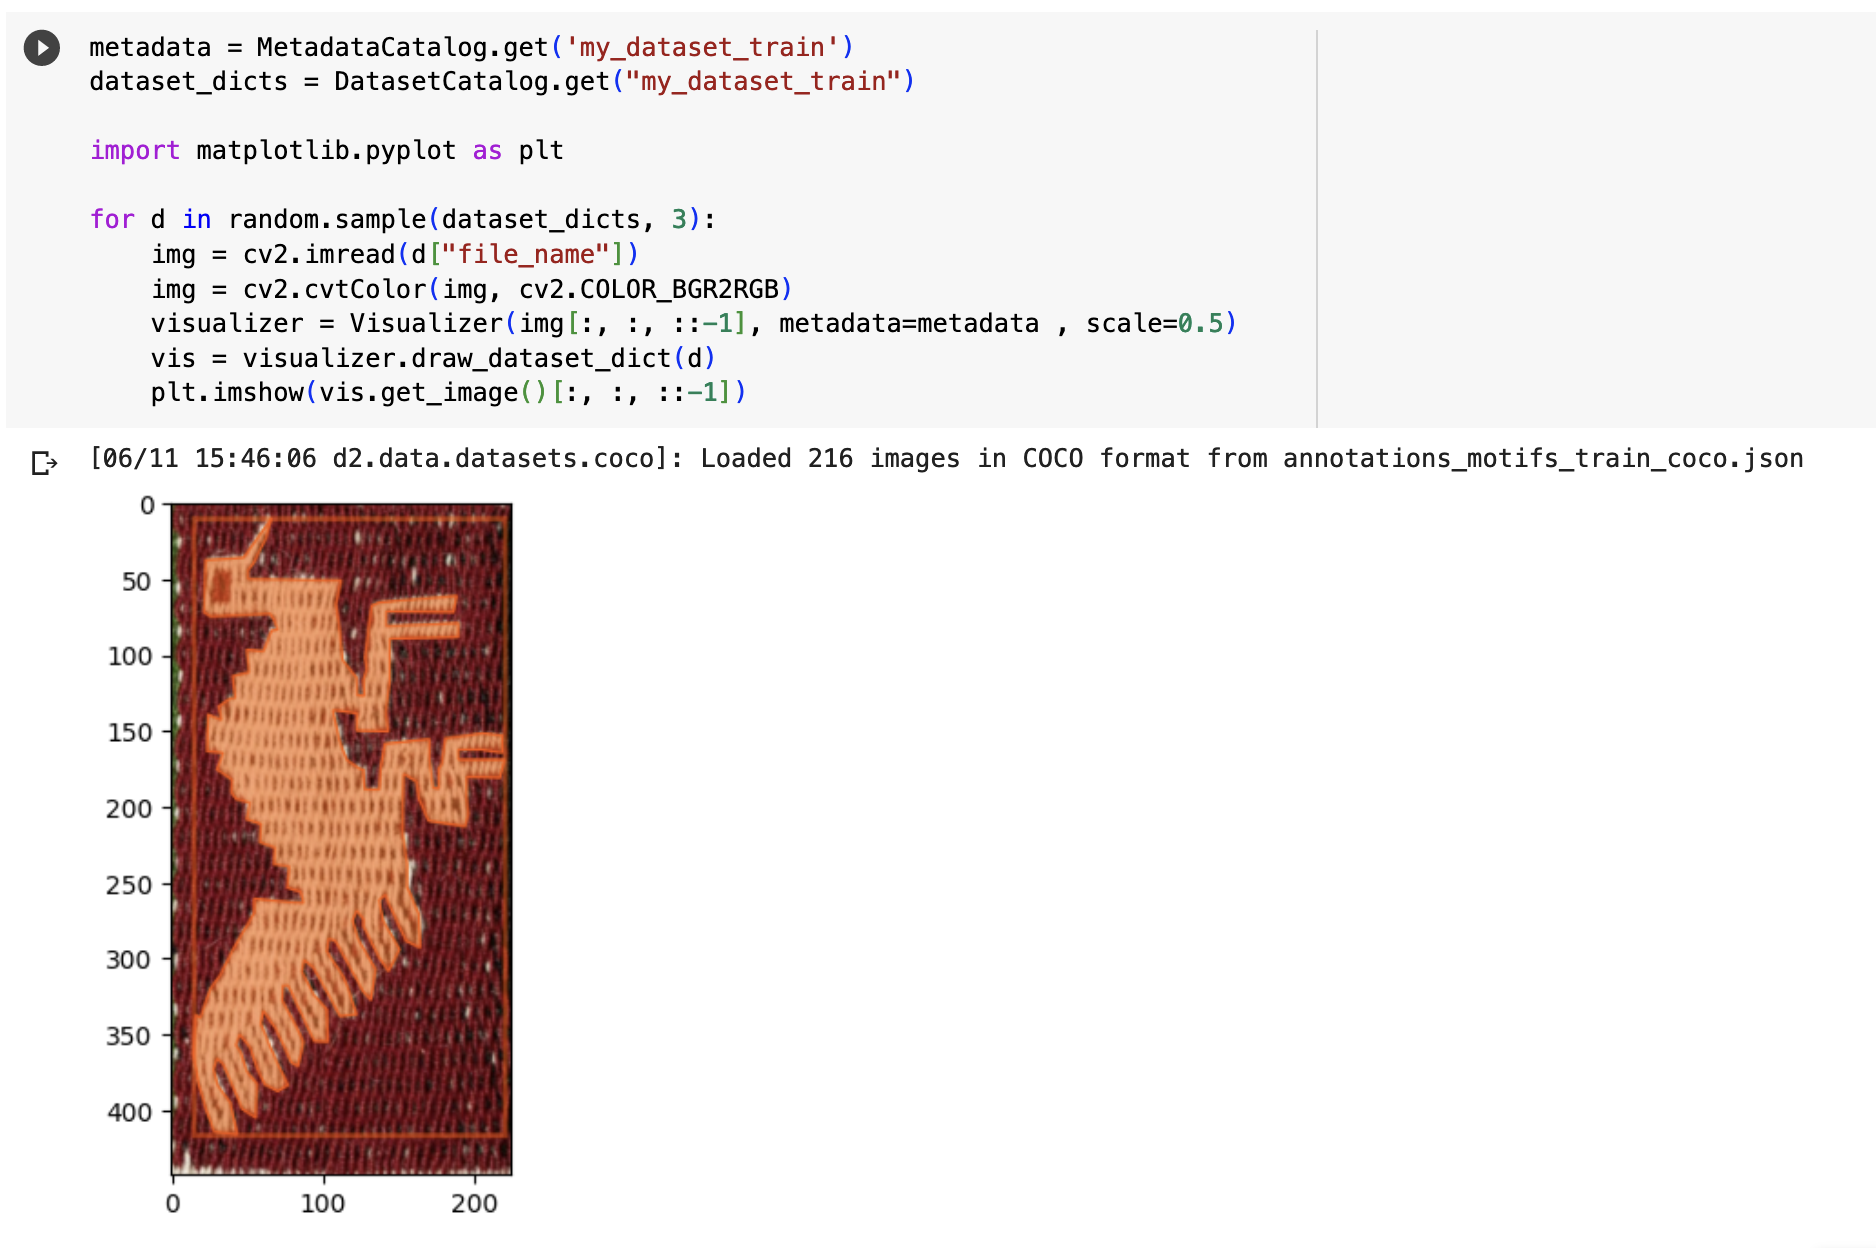
\includegraphics[width=15cm]{images/verifLecture.png}
    \caption{Capture d'écran du \textit{notebook} avec la lecture des annotations réalisée}
    \label{verifImgDetectron2} 
\end{figure}

Nous préparons ensuite l'entraînement du modèle. Pour cela, nous suivons les recommandations de la documentation de Detectron2. Nous utilisons notamment les fonctions du modèle zoo, un ensemble de fonctions prêtes à être utilisées pour créer l'architecture du modèle mais aussi les poids pré-entraînés de ce modèle. Il faut toutefois configurer un ensemble de paramètres, explicités ci-dessous : 

\begin{itemize}
    \item Le \textit{batch size}, littéralement \og taille du lot \fg, indique le nombre de données d'entraînement fourni au réseau à chaque itération. 
    \item La \textit{loss rate}, ou \og taux de perte\fg, est la différence entre le résultat attendu et le résultat de la prédiction du modèle. Au moment de la création du modèle, on indique à partir de quelle \textit{loss rate} l'entraînement peut s'arrêter (grâce à la commande cfg.SOLVER.BASE\_LR). On cherche à obtenir le taux de perte le plus faible possible. 
    \item La commande cfg.SOLVER.MAX\_ITER indique le nombre d'itérations à faire sur les données pour l'entraînement.
    \item Le \textit{RoI batch size} est la taille du lot de régions d'intérêt (RoI) qui sont testées au fur et à mesure du modèle pour calculer la \textit{loss rate}.
    \item La commande cfg.MODEL.ROI\_HEADS.NUM\_CLASSES indique le nombre de classes à chercher. Dans notre cas il n'y a qu'une classe : \og motif \fg.
\end{itemize}

\begin{figure}[!h]
    \centering
    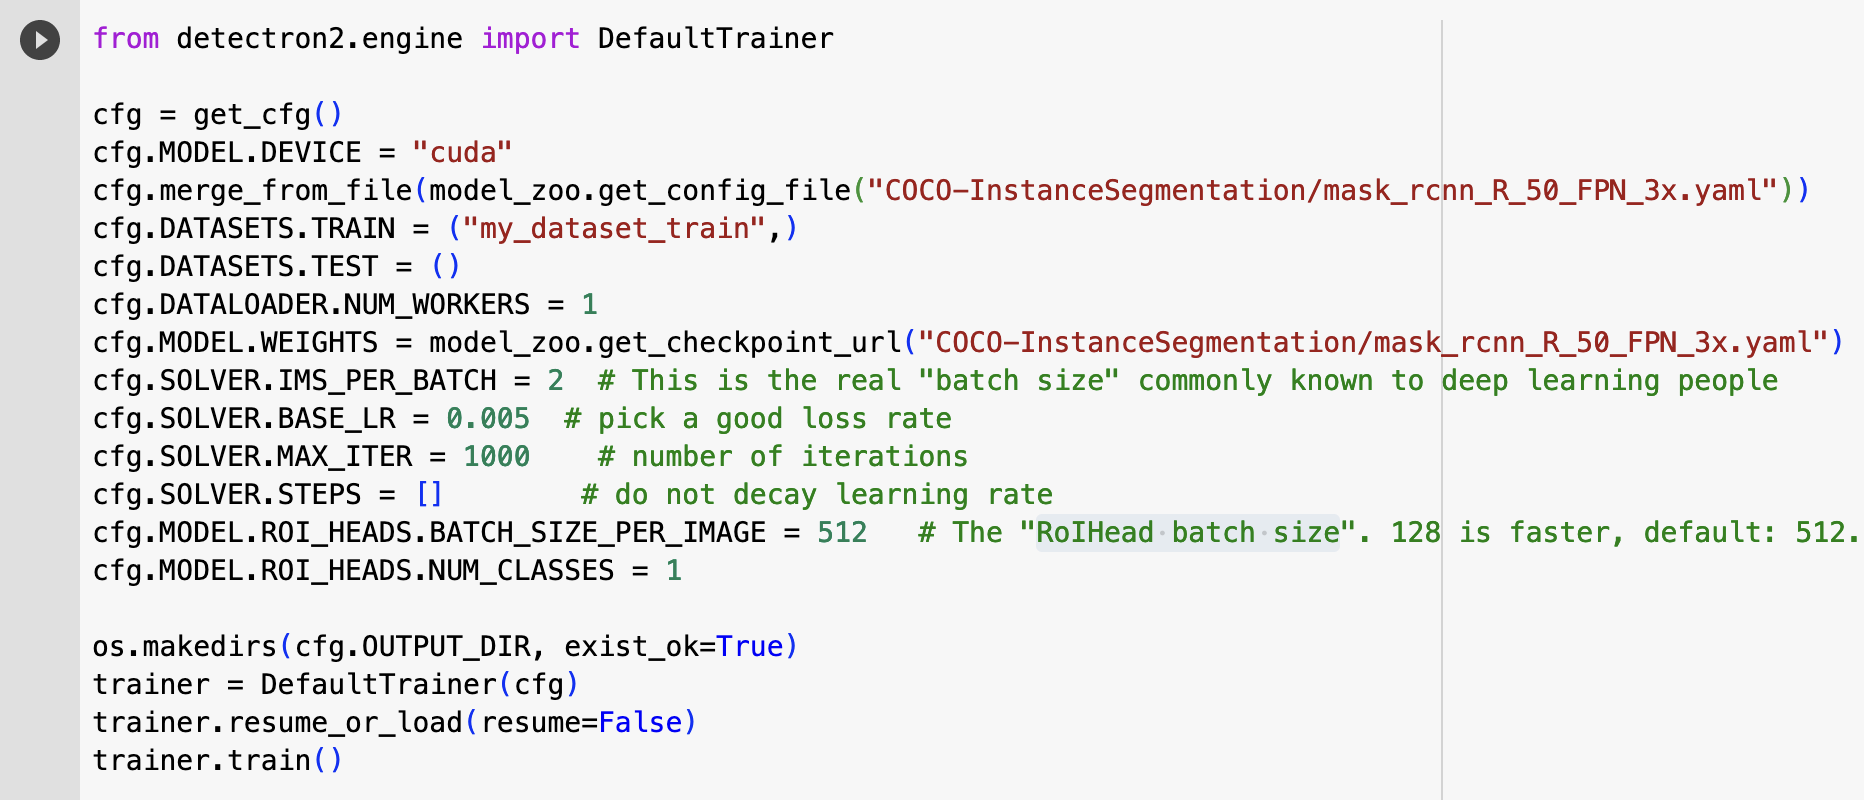
\includegraphics[width=16cm]{images/paramDetectron2.png}
    \caption{Paramètres du modèle entraîné}
    \label{paramDetectron2} 
\end{figure}

\section{Résultats}

La dernière partie du code contient une évaluation du modèle, elle renvoie un ensemble de métriques à partir de l'utilisation du modèle sur les données test. Une particularité de Detectron2 est qu'il prédit à la fois des \textit{bounding box} (cadre de sélection, aussi notés \textit{bbox}) c'est-à-dire un carré qui encadre le motif ou alors des masques de segmentation qui détoure les motifs. Ainsi, il est plus facile d'avoir une prédiction correcte en \textit{bbox} que d'obtenir une bonne segmentation de l'objet. 

Pour observer les résultats, on peut extraire certains visuels sur les données tests, c'est-à-dire une image ainsi que le masque produit par Detectron2 sur ce qu'il considère être un motif. Les résultats sont statistiquement corrects mais ils n'atteignent pas un niveau de prédiction parfait. Ainsi, pour certains motifs les contours du motif sont très bien détectés (voir l'image \ref{predViz}) alors que pour d'autres les \textit{bbox} sont correctes mais le détourage précis est inexact (voir l'image \ref{predVizAmbig}). 

\begin{figure}[!h]
    \centering
    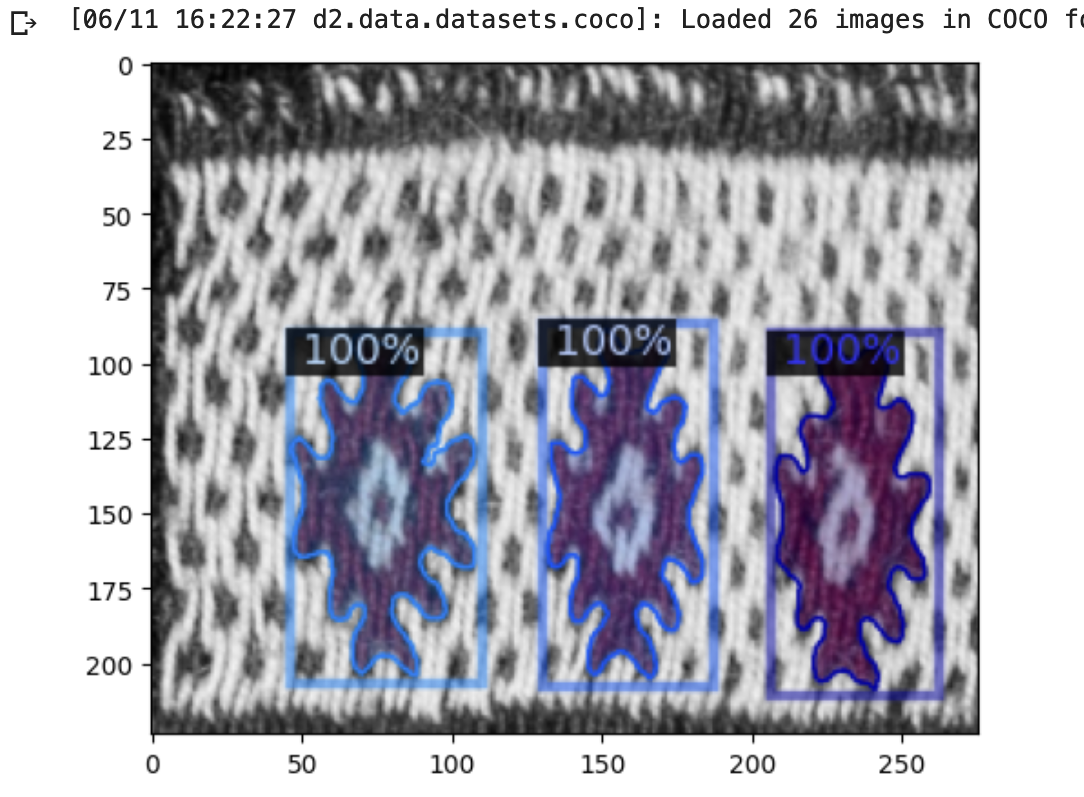
\includegraphics[width=13cm]{images/predViz3.png}
    \caption{Prédiction de motifs probante}
    \label{predViz} 
\end{figure}

\begin{figure}[!h]
    \centering
    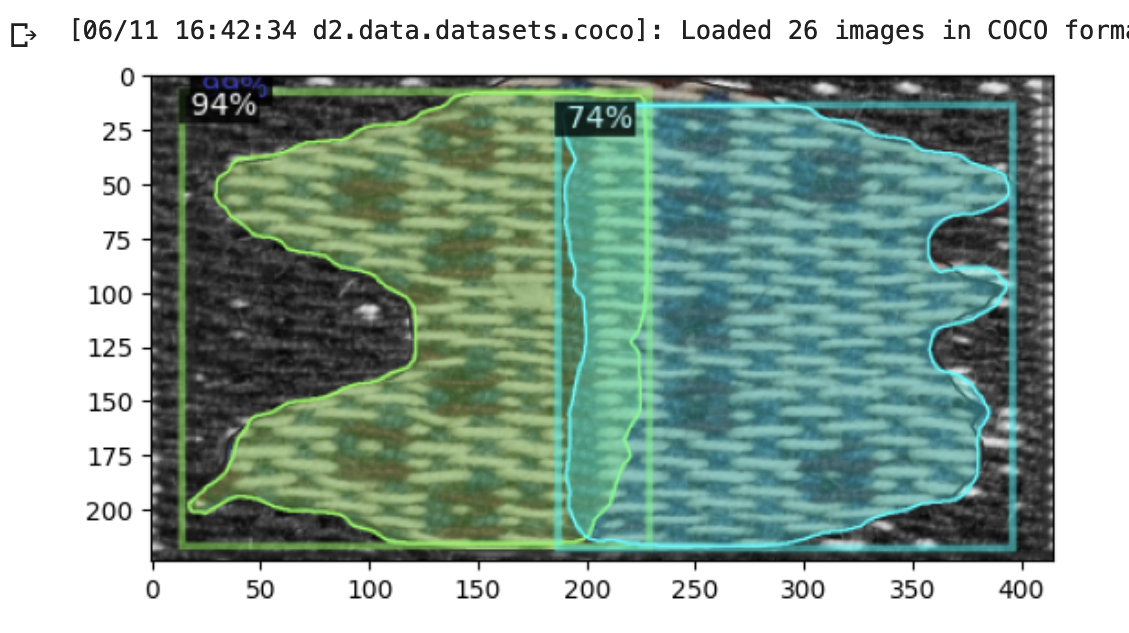
\includegraphics[width=13cm]{images/predVizAmbig.png}
    \caption{Prédiction de motif erronée}
    \label{predVizAmbig} 
\end{figure}

Dans ces exemples, le contraste entre le fond et le motif semble être discriminant. En effet, un contraste élevé semble faciliter la détection du motif.

Ces premières observations sont corroborées par les métriques d'évaluation du modèle obtenues. Dans un premier temps, il est possible d'observer la perte (\textit{loss}) au moment de l'apprentissage pour voir comment évolue l'écart entre le résultat attendu et le résultat de la prédiction du modèle. Cela permet aussi de vérifier que le modèle ne sur-apprend pas (\textit{overfitting}). On parle de surapprentissage du modèle quand celui-ci n'est plus capable de généraliser les prédictions à des données inconnues car il a trop \og vu\fg \:les données d'entraînement. Ainsi, il est possible de visualiser l'évolution de la perte au cours de l'apprentissage pour suivre le processus d'entraînement et de vérifier qu'elle se rapproche de 0.

\begin{figure}[!h]
    \centering
    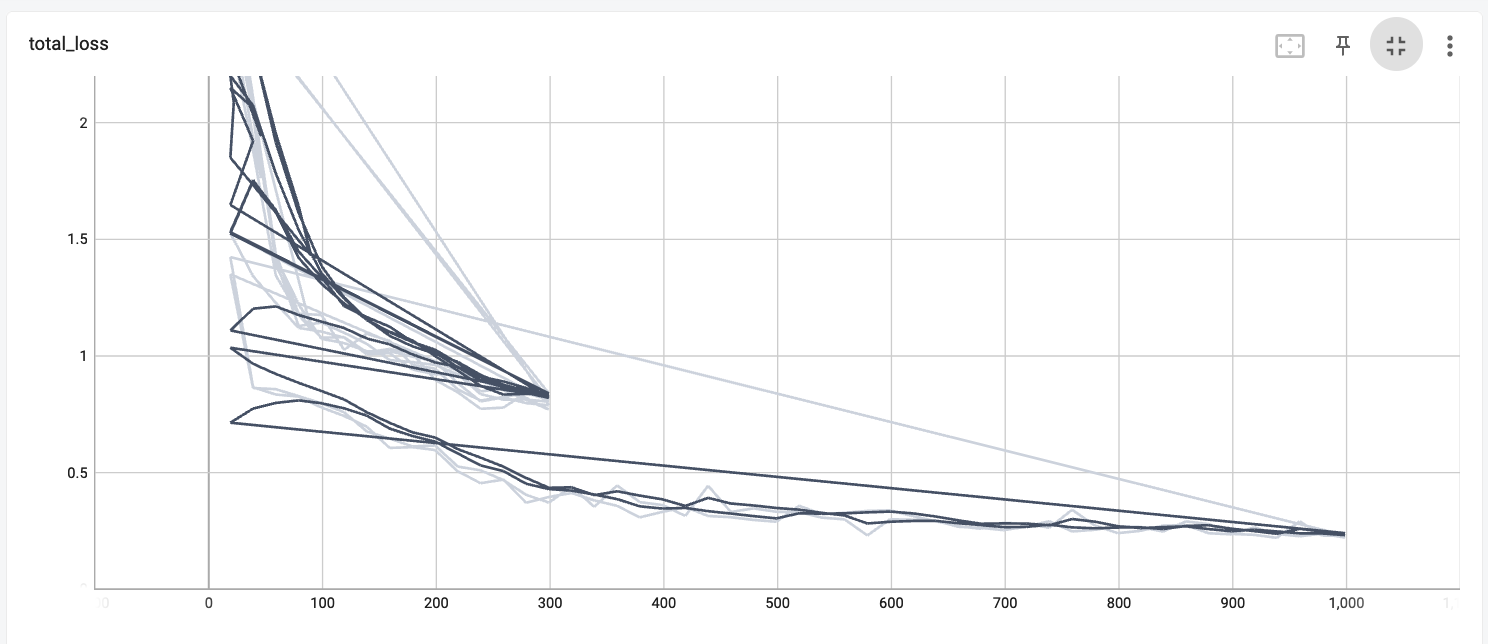
\includegraphics[width=16cm]{images/loss1000iter.png}
    \caption{Évolution de la perte durant l'entraînement du modèle}
    \label{lossIter} 
\end{figure}

\noindent Idéalement, la perte doit être inférieure à 0.5 voir 0.3. La perte totale à la fin de l'entraînement est de 0.264 ce qui est plutôt un bon résultat.

Par ailleurs, Detectron2 fournit des modules qui permettent d'obtenir des métriques plus précises après l'entraînement et la phase de test. Ces métriques se situent entre 0 et 100. Les résultats du modèle tel qu'il a été entraîné sont résumés dans le tableau suivant. 

\begin{table}[!h]
    \centering
    \begin{tabular}{|c|c|c|c|c|}
        \hline
        & \cellcolor{blue!20}\textbf{\textit{Average Precision} (AP)}& \cellcolor{blue!20} \textbf{AP 50} & \cellcolor{blue!20} \textbf{AP 75} & \cellcolor{blue!20} \textbf{AP \textit{loss}} \\ \hline \hline
         Bbox & 90.936 & 99.996 & 98.993 & 90.936 \\ \hline
         Segmentation & 69.203 & 99.996 & 90.409 & 69.203 \\ \hline
    \end{tabular}
    \caption{Résultat des métriques.}
    \label{tab:metrics}
\end{table}

La précision moyenne (\textit{average precision} ou \textit{mean average precision}) est la métrique la plus importante, elle indique la précision moyenne du modèle. Elle repose sur la notion de \textbf{précision}. La précision permet de quantifier la qualité d'un modèle, elle calcule le nombre de classes qui ont été correctement attribuées aux images. Elle est intrinsèquement liée aux notions de Vrai Positif (VP), Faux Positif (FP), Vrai Négatif (VN) et Faux Négatif (FN). Ces catégories contiennent l'ensemble des prédictions relativement à la réalité. 
\begin{itemize}
    \item Vrai Positif : les classes correctement reconnues par le modèle. 
    
    \textit{Exemple : les motifs qui sont détourés comme des motifs}.
    \item Faux Positif : les éléments qui sont reconnus comme appartenant à une classe alors qu'ils ne lui appartiennent pas 
    
    \textit{Exemple : les zones considérés comme des motifs alors qu'elles appartiennent au fond}.
    \item Vrai Négatif : les éléments qui sont reconnus comme n'appartenant pas à une classe et qui, effectivement, ne lui appartiennent pas 
    
    \textit{Exemple : les zones considérés comme le fond et qui sont effectivement hors des motifs}.
    \item Faux Négatif : les éléments qui sont reconnus comme n'appartenant pas à une classe alors qu'ils lui appartiennent 
    
    \textit{Exemple : les zones de motifs qui ne sont pas incluses à l'intérieur du motif détecté}.
\end{itemize}

La précision est ensuite calculée à partir du nombre d'éléments dans chaque catégorie selon l'équation suivante : 

\[\frac{VP}{VP+FP}\]

La précision moyenne est un peu plus compliquée puisqu'elle inclut le seuil de décision (\textit{s}) à partir duquel l'élément est considéré comme faisant partie de la classe. Ainsi, la précision moyenne calcule la précision pour différents seuils (1) dont elle fait la moyenne (2) . 

\[p(s) = \frac{VP(s)}{VP(s)+FP(s)} \hspace{40pt} (1)\] 

\[AP = \frac{1}{n} \sum_{i=1}^n p(s_i) \hspace{50pt} (2)\]

La précision moyenne est aussi calculée sur 50\% et 75\% de l'annotation initiale. Ainsi, si la prédiction correspond à 50\% de l'annotation, alors AP50 sera correcte. Dans notre cas, les précisions à 50\% et à 75\% nous indiquent que le modèle n'est pas complètement erroné mais qu'il perd en qualité sur 25\% des annotations, probablement sur les bordures des motifs d'après les visualisations obtenues. 
Enfin, la métrique d'AP-\textit{loss} permet de calculer la précision moyenne de la perte, elle calcule donc la capacité du modèle à apprendre et à s'adapter à l'échantillon d'apprentissage.

Idéalement, un modèle est considéré comme bon à partir d'une précision de 95\%. Toutefois, la documentation de Detectron2 indique qu'à partir de 70\% les résultats commencent à être corrects. Pour nos images, cela se traduit par la création de masques qui recouvrent uniquement une partie du motif, laissant de côté certaines parties réduites des motifs.

\section{Premières difficultés}

L'utilisation de Detectron2 nous a permis de réaliser une première analyse exploratoire en vision par ordinateur appliquée au textile. Nous pouvons déjà relever que malgré leur complexité --- et leur nom --- ces techniques de \og vision par ordinateur \fg (\textit{computer vision}) n'imitent pas encore parfaitement la capacité humaine à voir et analyser. C'est d'ailleurs pour cela que nous avons essayé de créer un corpus d'image équilibré, pour améliorer l'entraînement. Toutefois, les résultats sont déjà prometteurs puisque la reconnaissance des motifs se rapproche très fortement de celle réalisé par un \oe{}il humain pour une grande quantité d'images. 

Les performances du modèle pourraient être améliorées de plusieurs manières, d'une part le corpus d'entraînement reste un petit corpus. Entraîner le modèle sur une plus grande quantité d'images pourrait permettre d'en améliorer les capacités. Les images annotées étaient plutôt homogènes ce qui peut être un élément qui facilite la détection. Cependant, dans une logique d'élargissement du corpus, l'homogénéité peut devenir un défaut puisqu'elle pourrait limiter la reconnaissance des motifs tissés dont le style ou la technique sont proches mais différents. Ainsi, nous avons tout intérêt à élargir le corpus et à l'hétérogénéiser pour en améliorer ses performances. 

Les performances du modèle pourraient aussi être améliorées par une modification des annotations. Les images ont été découpées de telle sorte que elle ne contiennent qu'un seul rectangle qui, dans la grande majorité des cas, ne contenait qu'un motif. Il aurait pu être intéressant de récupérer, par exemple, des images contenant quatre rectangles contenant chacun un motif. D'autant plus que, bien souvent, sur les textiles les motifs se juxtaposent, voire se superposent. Cela pourrait permettre d'affiner la détection. \\

Par ailleurs, il aurait aussi pu être intéressant de modifier les caractéristiques colorimétriques des images pour essayer de saisir leur influence sur l'entraînement. Passer les images en niveau de gris ou bien diminuer le nombre de couleurs présentes dans l'image permettrait de vérifier si la couleur (et donc les valeurs des pixels) a un impact sur l'entraînement du modèle. Ce travail sur les couleurs peut se faire grâce au logiciel FIJI qui permet de récupérer des images en niveau de gris. Il permet aussi d'obtenir une visualisation des couleurs en 3D grâce à la quantification des couleurs WuQuant et de faire varier le nombre de couleurs présentes dans l'image.

Comme nous pouvons voir sur l'image, la modification du nombre de couleurs peut se faire de telle sorte que cela ne modifie pas l'image pour l'\oe{}il humain. Sur l'image \ref{couleur}, nous sommes passés de 256 couleurs à 15 couleurs. Les valeurs des pixels ont donc été largement diminuées ce qui pourrait simplifier le traitement des images au moment de l'apprentissage et améliorer la détection de motifs. Cela reste à vérifier.

\begin{figure}[!h]
    \begin{minipage}[c]{.5\linewidth}
            \begin{center}
                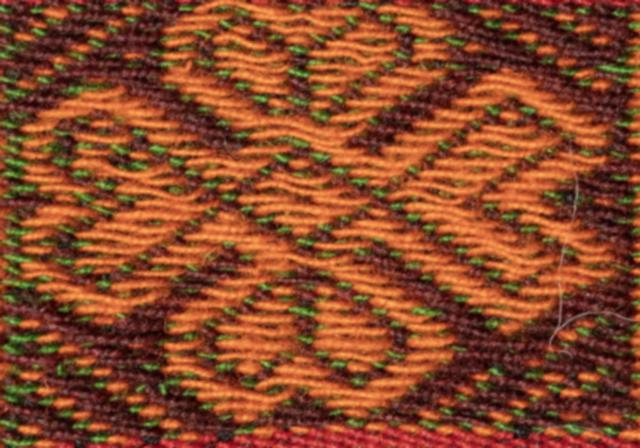
\includegraphics[width=7cm]{images/A1_F07.jpg}
            \end{center}
    \end{minipage}
    \begin{minipage}[c]{.5\linewidth}
        \begin{center}
            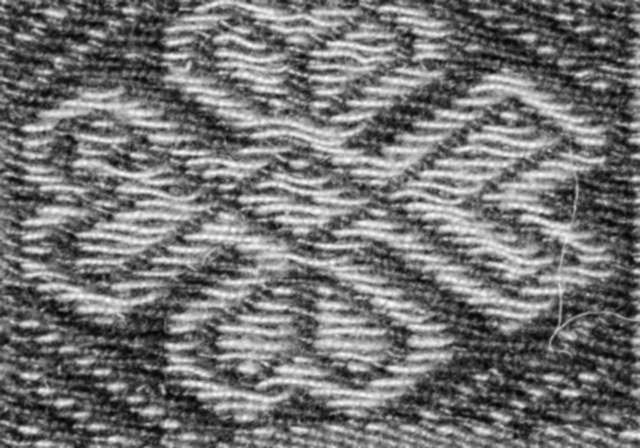
\includegraphics[width=7cm]{images/A1_F07_16bits.jpg}
        \end{center}
    \end{minipage}
    \caption{Image A1\_F07 en RGB et en 16-bits}
\end{figure}

\begin{figure}[!h]
    \begin{center}
    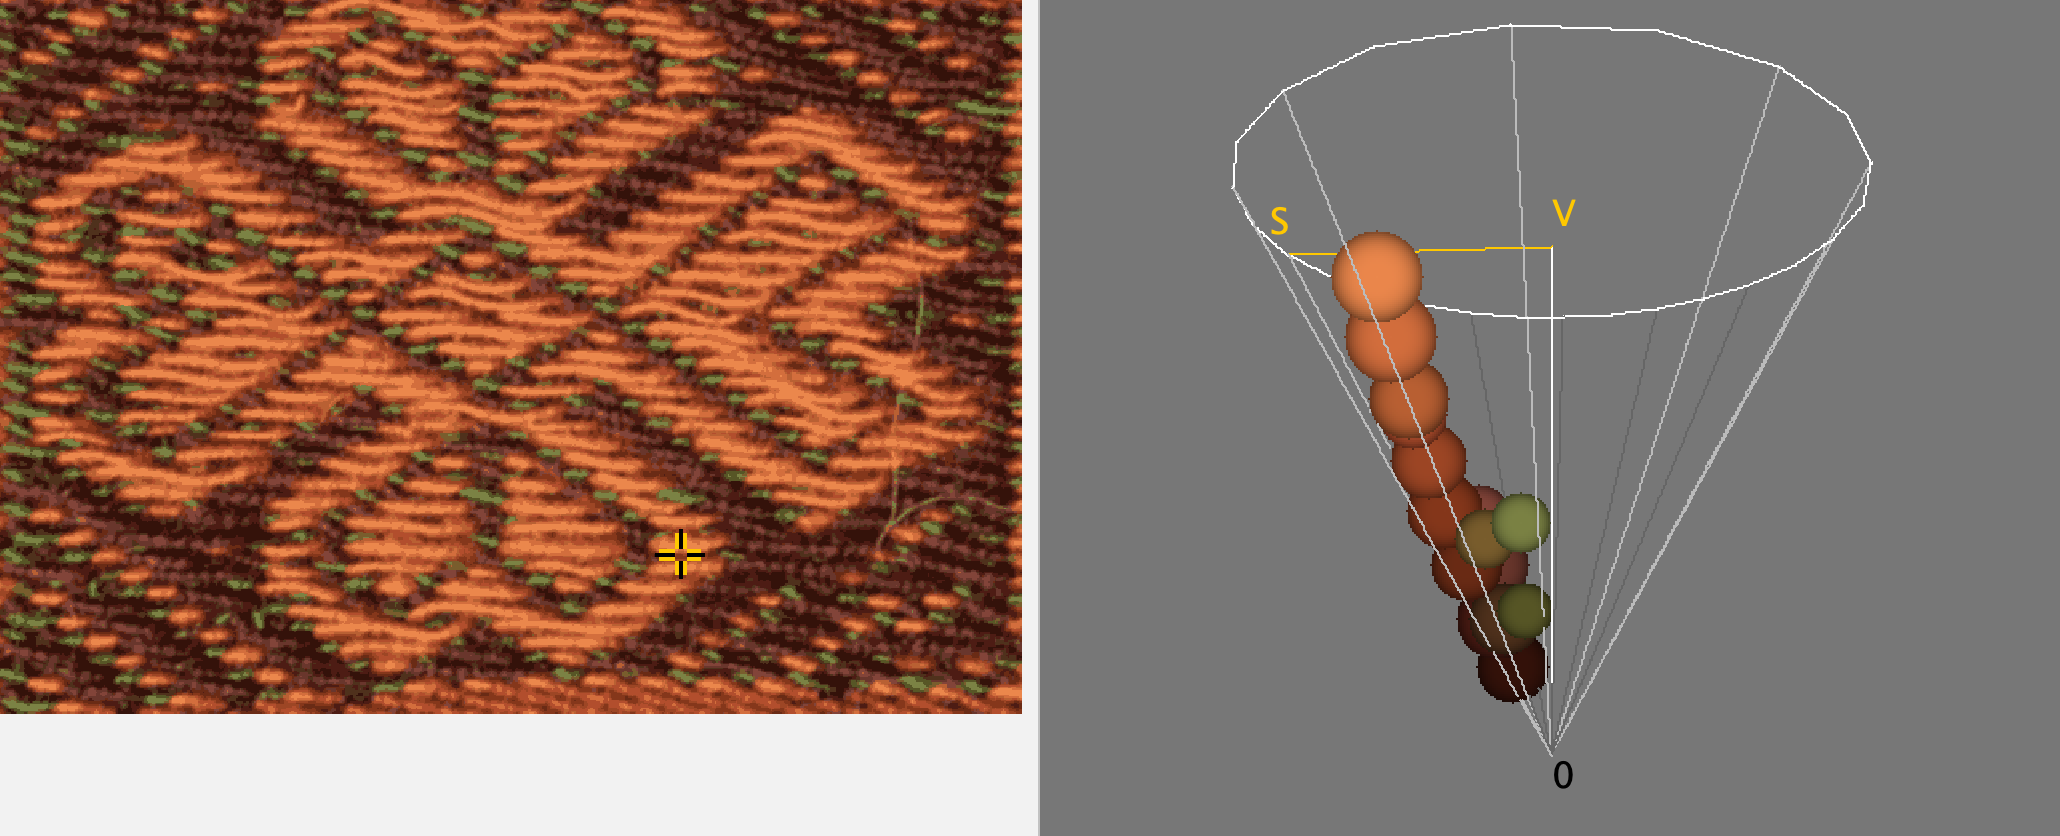
\includegraphics[width=16cm]{images/WuQuant_15col.png}
    \caption[\textit{Color Inspector 3D}]{ Même image dans le \textit{Color Inspector 3D} de FIJI avec réduction du nombre de couleurs présentes dans l'image}
    \label{couleur}
    \end{center}
\end{figure}






\chapter{Suites de la recherche}

\section{Poursuite dans la détection des motifs}

Dans un premier temps, et dans la continuité du travail réalisé, il sera possible d'améliorer la détection de motifs. Pour cela, nous pourrons prendre en compte toutes les suggestions spécifiées dans la partie précédente. 

Pour élargir le corpus, il serait intéressant de réaliser un \textit{web scrapping} (récupération de données en ligne) de la base de données \og \textit{Weaving Communities of Practice} \fg \:qui contient des images de textiles andins. Comme nous l'avons expliqué, le musée Amano à Lima -- musée des textiles précolombiens -- ont mis en ligne des images dans le cadre du projet \textit{Google Art \& Culture}. Toutefois, le manque de métadonnées rend impossible l'utilisation telle quelle des données disponibles. Je souhaite donc contacter les musées Larco et Amano de Lima pour voir s'il serait possible de récupérer des photographies des pièces textiles de leurs collections. 

Élargir le corpus implique aussi la création d'un système d'organisation pour pouvoir référencer les textiles qui viennent de sources différentes et qui ont des composantes spatio-temporelles et techniques différentes. Ainsi, le logiciel Tropy me semble être un outil adapté puisqu'il permet d'archiver et d'organiser des images ainsi que leurs métadonnées.

Il s'agirait alors d'annoter certaines images pour recommencer le processus réalisé en master 1. L'annotation pourrait se faire de manière plus fine afin de distinguer différentes catégories comme les motifs géométriques, anthropomorphes ou de faune et de flore. Ces catégories extraites pourraient donner une idée des variations des motifs dans le temps et dans l'espace, et ainsi permettre une comparaison aux travaux déjà réalisés sur la question. 

\section{La spatialisation des images}

La spatialisation des textiles et de leurs images semble être une hypothèse de recherche cohérente par rapport aux données dont nous disposons. Ainsi, la spatialisation permettrait de venir questionner les influences entre les différents groupes producteurs de textiles dans les foyers de civilisation péruviens afin de comprendre les \og phénomènes de diffusion, d'innovation et de blocage technique \fg \:dont parle Sophie Desrosiers\footcite[p.~264]{desrosiersTechniquesTissageOntelles2010}. En effet, la proximité géographique ou temporelle de groupes ethniques n'implique pas forcément la diffusion de techniques et d'iconographies. Les circulations des textiles et de leurs techniques ont pu se faire sur de longues distances, notamment lors de migrations entre la côte et les Andes.

\noindent Comme le soulignent Carmen Brando et son équipe dans un article de 2021, 

\begin{quote}
    \og  À partir des années 1970 [...] les systèmes d'information géographique (SIG) progressent et se propagent depuis la géographie numérique vers les disciplines connexes (histoire, archéologie, etc.), démontrant ainsi l'intérêt et l'utilité de l'analyse spatiale et de son intégration dans la \og boîte à outils \fg \:des praticiens du numérique en SHS \fg \footcite[p.~3]{brandoIntroductionHumanitesNumeriques2021}. 
\end{quote} 

\noindent Ainsi, il pourrait être intéressant de se pencher sur l'implémentation d'un système d'information géographique organisant des textiles andins. La création d'une base de données sur Tropy pourrait permettre de récupérer des informations géographiques et donc de cartographier les pièces en présence. Toutefois, les objets ne sont pas fixes et peuvent bouger au cours de leur existence. On peut notamment penser aux pièces textiles créées pour les enfants sacrifiés. Retrouvés sur les plus hauts sommets des Andes, les tombes de ces momies contiennent des pièces qui ont probablement été conçues dans des provinces très éloignées comme en atteste la présence de plumes d'oiseaux amazoniens ou de coquillages dans les sépultures\footcite{abalderussoArteTextilIncaico2010}. Il faut alors se questionner sur la localisation des pièces. Le lieu de découverte est souvent le seul dont on dispose mais il est parfois trompeur sur l'origine de la technique. \\

D'autre part, le \textit{Google Art\&Culture Experiments} a proposé différents projets de cartographie ou de spatialisation d'\oe{}uvres d'art suivant un axe artistique et iconographique\footnote{\url{https://experiments.withgoogle.com/collection/arts-culture}, consulté le 03/01/2023}. Certains projets s'inscrivent dans une logique d'histoire de l'art ou de muséalité.
\begin{itemize}
    \item Le projet \textit{t-SNE maps} \footnote{\url{https://experiments.withgoogle.com/t-sne-map}, consulté le 03/01/2023} propose, via de l'apprentissage machine, une carte 3D qui organise des \oe{}uvres d'art selon leur similarité visuelle (donc sans utiliser de métadonnées).
\end{itemize}

\noindent Ce projet renvoie à un nouvel axe de la recherche (les premiers travaux datent des cinq dernières années) en humanités numériques : l'utilisation de la réduction de dimension pour classer des images, en utilisant un algorithme \textit{t-SNE} ou \textit{Uniform Manifold Approximation and Projection} (algorithme UMAP)\footnote{La publication suivante reprend précisément en quoi consiste mathématique et informatiquement le UMAP : \cite{mcinnesUMAPUniformManifold2018}}. UMAP (\textit{Uniform Manifold Approximation \& Projection}) est un algorithme de réduction non-linéaire de dimension\footnote{\url{https://umap-learn.readthedocs.io/en/latest/index.html} est le site de référence quant au UMAP. On y trouve aussi le lien Git Hub qui permet d'implémenter l'algorithme en langage Python}. Son but est de représenter des données en une plus faible dimension qui présente la même topologie que le nuage des observations dans l'espace de départ. C'est un algorithme qui a d'abord été développé en biologie. Il repose sur la création de matrices de similarités. Pour obtenir des matrices où chaque rang est une image et chaque colonne une information, nous pouvons utiliser un réseau de neurone convolutif (ou CNN). Un des premiers UMAP développés est le Fashion MNIST \footnote{\url{https://observablehq.com/@stwind/exploring-fashion-mnist}, consulté le 03/01/2023}  créé à partir d'une base de donnée de vêtements (issue du site de vente en ligne Zalando) et qui classe les items selon leur ressemblance (T-shirt, pantalon, chaussures etc.). De nombreuses expérimentations de ce type de spatialisation d'images sont en cours. 

Une modélisation en cluster via UMAP\footnote{Les algortihmes t-SNE et UMAP reposent sur les mêmes logiques de spatialisation, le modèle UMAP a tendance à créer des clusters plus distincts que le t-SNE qui met en avant la continuité entre les données. \cite[p.~30]{mcinnesUMAPUniformManifold2018}.} à partir des similarités iconographiques des pièces textiles pourrait permettre de saisir les variations des motifs.  On peut suivre ce qui a été développé par D. Clermont sur l'entraînement de réseau de neurones convolutifs (CNN) appliqué à des échantillons de soie dans le cadre du projet SilkNow. Il propose \og d'entraîner un CNN à fournir des caractéristiques similaires pour des images d'entrées similaires et des caractéristiques différentes pour des images différentes, de sorte que la distance euclidienne des vecteurs de caractéristiques puisse être utilisée pour mesurer la similarité entre des paires d'images\fg \footcite[p.~642]{clermontAssessingSemanticSimilarity2020}. Le processus de convolution permet de garder un maximum d'informations sur l'image (notamment les couleurs) et de venir attribuer un poids aux images. À partir de cela, il serait possible de constituer une matrice analysée par le UMAP afin de spatialiser les images en fonction de leur similarité. L'idée étant de trouver les images qui ont le plus de similarités et de les rassembler en clusters dans un espace 3D, comme proposé pour le projet Fashion MNIST.

\chapter*{Conclusion}
\addcontentsline{toc}{chapter}{Conclusion}
\pagestyle{empty}

Les premiers résultats que nous avons obtenus sur ce corpus réduit ébauchent des perspectives intéressantes pour la suite.\\

Après une longue phase de préparation de données, nous avons pu tester le modèle Detectron2 sur le corpus d'images annotées que nous avions créé. Malgré les spécificités de la technique textile, le modèle a réussi à obtenir une précision moyenne de près de 91\% pour les cadres de sélection et de 69\% pour la segmentation des motifs. Ces résultats sont corrects mais il reste de nombreux points d'amélioration. 

D'une part, il faudrait augmenter la quantité de données tout en augmentant l'hétérogénéité pour améliorer les capacités du modèle sur un corpus plus large. En outre, le travail sur les couleurs ou la dimension des images pourrait aussi être une piste à développer pour améliorer le modèle. Pour cela, il s'agira aussi de renforcer nos connaissances et nos lectures sur le côté technique de l'apprentissage machine.

D'autre part, il faudrait retravailler sur les annotations pour obtenir une classification plus fine des motifs. Nous pourrions utiliser des métriques supplémentaires pour essayer de comprendre les facteurs qui influencent le plus l'entraînement et les capacités du modèle. \\

Malgré leur spécificité technique, les textiles andins, s'ils sont annotés correctement, semblent pouvoir être classifiés automatiquement. Cette classification pourrait permettre, à terme, une analyse spatiale des pièces textiles à travers leurs techniques et leur iconographie. Ainsi, la détection de motifs par les réseaux de neurones n'est pas la seule information qui pourrait être analysée. La prise en compte du lieu de production ou de découverte des techniques pourrait être intéressante pour visualiser les dynamiques de circulation de ces textiles. 

Par ailleurs, les dernières avancées en analyse d'image nous poussent à réfléchir en terme de méthodes non-supervisées telles que la réduction de dimension (par exemple grâce à l'algorithme UMAP) pour visualiser et penser les textiles dans les Andes. Cette visualisation pourrait aussi apporter un élément de réflexion en plus aux nombreuses études qui portent sur la classification des techniques textiles.

\listoffigures

\clearpage 

\chapter*{Bibliographie}
\addcontentsline{toc}{chapter}{Bibliographie}

\printbibliography[heading=subbibintoc,keyword=TextAnd,title=Textiles]
\printbibliography[heading=subbibintoc, keyword=textnum,title=Humanités Numériques]
\printbibliography[heading=subbibintoc, title=Sitographie, type=online]

\end{document}

